\documentclass[a4paper,justified,final,twoside,nobib]{tufte-book}

\hypersetup{colorlinks}% uncomment this line if you prefer colored hyperlinks (e.g., for onscreen viewing)

\usepackage{mathtools} %added mathtools for piecewise functions

%%
% Book metadata
\title{A\\Machine Learning\\Handbook\thanks{Thanks to Edward R.~Tufte for his inspiration.}}
\author[]{}
\publisher{Publisher of This Book}

%%
% Automated bibliography management
\usepackage{natbib}
\setcitestyle{authoryear}

%%
% If they're installed, use Bergamo and Chantilly from www.fontsite.com.
% They're clones of Bembo and Gill Sans, respectively.
%\IfFileExists{bergamo.sty}{\usepackage[osf]{bergamo}}{}% Bembo
%\IfFileExists{chantill.sty}{\usepackage{chantill}}{}% Gill Sans

\usepackage{microtype}

%%
% Describe algorithms using fancy pseudo code
\usepackage{algorithm}
\usepackage[noend]{algpseudocode}

%%
% Just some sample text
\usepackage{lipsum}
\usepackage{soul}
%%
% For nicely typeset tabular material
\usepackage{booktabs}
\usepackage{pdfpages}

%%
% For graphics / images
\usepackage{graphicx}
\setkeys{Gin}{width=\linewidth,totalheight=\textheight,keepaspectratio}
\graphicspath{{graphics/}}

% The fancyvrb package lets us customize the formatting of verbatim
% environments.  We use a slightly smaller font.
\usepackage{fancyvrb}
\fvset{fontsize=\normalsize}

%%
% Prints argument within hanging parentheses (i.e., parentheses that take
% up no horizontal space).  Useful in tabular environments.
\newcommand{\hangp}[1]{\makebox[0pt][r]{(}#1\makebox[0pt][l]{)}}

%%
% Prints an asterisk that takes up no horizontal space.
% Useful in tabular environments.
\newcommand{\hangstar}{\makebox[0pt][l]{*}}

%%
% Prints a trailing space in a smart way.
\usepackage{xspace}
% bold in maths equations
\usepackage{bm}

%%
% Some shortcuts for Tufte's book titles.  The lowercase commands will
% produce the initials of the book title in italics.  The all-caps commands
% will print out the full title of the book in italics.
\newcommand{\vdqi}{\textit{VDQI}\xspace}
\newcommand{\ei}{\textit{EI}\xspace}
\newcommand{\ve}{\textit{VE}\xspace}
\newcommand{\be}{\textit{BE}\xspace}
\newcommand{\VDQI}{\textit{The Visual Display of Quantitative Information}\xspace}
\newcommand{\EI}{\textit{Envisioning Information}\xspace}
\newcommand{\VE}{\textit{Visual Explanations}\xspace}
\newcommand{\BE}{\textit{Beautiful Evidence}\xspace}
\newcommand{\ics}{\smallcaps{ICS5110 Applied Machine Learning\xspace}}

\newcommand{\TL}{Tufte-\LaTeX\xspace}

% Prints the month name (e.g., January) and the year (e.g., 2008)
\newcommand{\monthyear}{%
  \ifcase\month\or January\or February\or March\or April\or May\or June\or
  July\or August\or September\or October\or November\or
  December\fi\space\number\year
}

% Prints an epigraph and speaker in sans serif, all-caps type.
\newcommand{\openepigraph}[2]{%
  %\sffamily\fontsize{14}{16}\selectfont
  \begin{fullwidth}
  \sffamily\large
  \begin{doublespace}
  \noindent\allcaps{#1}\\% epigraph
  \noindent\allcaps{#2}% author
  \end{doublespace}
  \end{fullwidth}
}

% Inserts a blank page
\newcommand{\blankpage}{\newpage\hbox{}\thispagestyle{empty}\newpage}

\usepackage{units}

% Typesets the font size, leading, and measure in the form of 10/12x26 pc.
\newcommand{\measure}[3]{#1/#2$\times$\unit[#3]{pc}}

% Macros for typesetting the documentation
\newcommand{\hlred}[1]{\textcolor{Maroon}{#1}}% prints in red
\newcommand{\hangleft}[1]{\makebox[0pt][r]{#1}}
\newcommand{\hairsp}{\hspace{1pt}}% hair space
\newcommand{\hquad}{\hskip0.5em\relax}% half quad space
\newcommand{\TODO}{\textcolor{red}{\bf TODO!}\xspace}
\newcommand{\ie}{\textit{i.\hairsp{}e.}\xspace}
\newcommand{\eg}{\textit{e.\hairsp{}g.}\xspace}
\newcommand{\na}{\quad--}% used in tables for N/A cells
\providecommand{\XeLaTeX}{X\lower.5ex\hbox{\kern-0.15em\reflectbox{E}}\kern-0.1em\LaTeX}
\newcommand{\tXeLaTeX}{\XeLaTeX\index{XeLaTeX@\protect\XeLaTeX}}
% \index{\texttt{\textbackslash xyz}@\hangleft{\texttt{\textbackslash}}\texttt{xyz}}
\newcommand{\tuftebs}{\symbol{'134}}% a backslash in tt type in OT1/T1
\newcommand{\doccmdnoindex}[2][]{\texttt{\tuftebs#2}}% command name -- adds backslash automatically (and doesn't add cmd to the index)
\newcommand{\doccmddef}[2][]{%
  \hlred{\texttt{\tuftebs#2}}\label{cmd:#2}%
  \ifthenelse{\isempty{#1}}%
    {% add the command to the index
      \index{#2 command@\protect\hangleft{\texttt{\tuftebs}}\texttt{#2}}% command name
    }%
    {% add the command and package to the index
      \index{#2 command@\protect\hangleft{\texttt{\tuftebs}}\texttt{#2} (\texttt{#1} package)}% command name
      \index{#1 package@\texttt{#1} package}\index{packages!#1@\texttt{#1}}% package name
    }%
}% command name -- adds backslash automatically
\newcommand{\doccmd}[2][]{%
  \texttt{\tuftebs#2}%
  \ifthenelse{\isempty{#1}}%
    {% add the command to the index
      \index{#2 command@\protect\hangleft{\texttt{\tuftebs}}\texttt{#2}}% command name
    }%
    {% add the command and package to the index
      \index{#2 command@\protect\hangleft{\texttt{\tuftebs}}\texttt{#2} (\texttt{#1} package)}% command name
      \index{#1 package@\texttt{#1} package}\index{packages!#1@\texttt{#1}}% package name
    }%
}% command name -- adds backslash automatically
\newcommand{\docopt}[1]{\ensuremath{\langle}\textrm{\textit{#1}}\ensuremath{\rangle}}% optional command argument
\newcommand{\docarg}[1]{\textrm{\textit{#1}}}% (required) command argument
\newenvironment{docspec}{\begin{quotation}\ttfamily\parskip0pt\parindent0pt\ignorespaces}{\end{quotation}}% command specification environment
\newcommand{\docenv}[1]{\texttt{#1}\index{#1 environment@\texttt{#1} environment}\index{environments!#1@\texttt{#1}}}% environment name
\newcommand{\docenvdef}[1]{\hlred{\texttt{#1}}\label{env:#1}\index{#1 environment@\texttt{#1} environment}\index{environments!#1@\texttt{#1}}}% environment name
\newcommand{\docpkg}[1]{\texttt{#1}\index{#1 package@\texttt{#1} package}\index{packages!#1@\texttt{#1}}}% package name
\newcommand{\doccls}[1]{\texttt{#1}}% document class name
\newcommand{\docclsopt}[1]{\texttt{#1}\index{#1 class option@\texttt{#1} class option}\index{class options!#1@\texttt{#1}}}% document class option name
\newcommand{\docclsoptdef}[1]{\hlred{\texttt{#1}}\label{clsopt:#1}\index{#1 class option@\texttt{#1} class option}\index{class options!#1@\texttt{#1}}}% document class option name defined
\newcommand{\docmsg}[2]{\bigskip\begin{fullwidth}\noindent\ttfamily#1\end{fullwidth}\medskip\par\noindent#2}
\newcommand{\docfilehook}[2]{\texttt{#1}\index{file hooks!#2}\index{#1@\texttt{#1}}}
\newcommand{\doccounter}[1]{\texttt{#1}\index{#1 counter@\texttt{#1} counter}}

% Generates the index
\usepackage{makeidx}
\makeindex

\usepackage{tikz}
\usepackage{makecell}

\begin{document}
%% Cover Page
\begingroup
\thispagestyle{empty}
\begin{tikzpicture}[remember picture,overlay]
\node[inner sep=0pt, outer sep=0pt] (background) at (current page.center) {\includegraphics[width=\paperwidth]{cover/cover_oreilly_style.pdf}};
\end{tikzpicture}
\vfill
\endgroup

% Front matter
\frontmatter

% r.3 full title page
%% \maketitle


% v.4 copyright page
\newpage
\begin{fullwidth}
~\vfill
\thispagestyle{empty}
\setlength{\parindent}{0pt}
\setlength{\parskip}{\baselineskip}
\begin{figure*}[h]
	\includegraphics[width=2.5in]{UMLOGO_redRGB.png}%
\end{figure*}

\par Copyright \copyright\ \the\year\ \ics\ class of 2018/9, University of Malta.


\par\smallcaps{Jean-Paul Ebejer, Dylan Seychell, Lara Marie Demajo, Daniel Farrugia, Keith Mintoff, Franco Cassar Manghi, David Farrugia, Ivan Salomone, Andrew Cachia, Jake J.\ Dalli, Joseph Azzopardi, Natalia Mallia, Mark Muscat, Stefan Cassar, George Eduardo Buckup Sulzbeck \hl{ADD YOUR NAME TO THIS LIST}} %TODO


\par Licensed under the Apache License, Version 2.0 (the ``License''); you may not
use this file except in compliance with the License. You may obtain a copy
of the License at \url{http://www.apache.org/licenses/LICENSE-2.0}. Unless
required by applicable law or agreed to in writing, software distributed
under the License is distributed on an \smallcaps{``AS IS'' BASIS, WITHOUT
WARRANTIES OR CONDITIONS OF ANY KIND}, either express or implied. See the
License for the specific language governing permissions and limitations
under the License.\index{license}

\par\textit{First printing, \monthyear}
\end{fullwidth}

% r.5 contents
\tableofcontents

%%\listoffigures

%%\listoftables

% r.9 introduction
\cleardoublepage
\chapter{Introduction}

This book explains popular Machine Learning terms.  We focus to explain each term comprehensively, through the use of examples and diagrams.  The description of each term is written by a student sitting in for \ics\footnote{\url{https://www.um.edu.mt/courses/studyunit/ICS5110}} at the University of Malta (class 2018/2019).  This study-unit is part of the MSc.\ in AI offered by the Department of Artificial Intelligence, Faculty of ICT.

%%
% Start the main matter (normal chapters)
\mainmatter

%% JP's example file -- file must be stored in directory "terms" and have
%% the term and initials of the student in the filename.
\chapter[Activation Functions]{Activation Functions}
\label{ch:activation-functions}\index{activation functions|(}
\citet{caterini2018} defined artificial neural networks as ``a model that would imitate the function of the human brain---a set of neurons joined together by a set of connections. Neurons, in this context, are composed of a weighted sum of their inputs followed by a nonlinear function, which is also known as an activation function.''

Activation functions are used in artificial neural networks to determine whether the output of the neuron should be considered further or ignored. If the activation function chooses to continue considering the output of a neuron, we say that the neuron has been activated. The output of the activation function is what is passed on to the subsequent layer in a multilayer neural network. To determine whether a neuron should be activated, the activation function takes the output of a neuron and transforms it into a value commonly bound to a specific range, typically from 0 to 1 or -1 to 1 depending on the which activation function is applied.

\section{Step Function}\label{sec:step-function}\index{step function}

\begin{marginfigure}
  \includegraphics{graphics/activation_functions/step_function.png}
  \caption{
    A graph of the step function. 
  }
  \label{fig:stepfunction}
\end{marginfigure}

\begin{equation}\label{stepfunction}
    f(x) =
    \begin{dcases*}
        0 & \text{for \(x < 0\)} \\
        1 & \text{for \(x \geq 0\)} \\
    \end{dcases*}
\end{equation}

\begin{equation}\label{stepfunctionderivative}
    \frac{d}{d(x)}f(x) =
      \begin{dcases*}
                                       0 & \text{for \(x \neq 0\)} \\
                                       ? & \text{for \(x = 0\)} \\
      \end{dcases*}
\end{equation}

The Heavside step function, visualised in figure~\ref{fig:stepfunction} and defined by equation~\ref{stepfunction}, is one of the simplest activation functions that can be used in a neural network. This function returns 0 if the input of a node is less than a predetermined threshold (typically 0), or otherwise it returns 1 if the output of the node is greater than or equal to the threshold. This activation function was first used in a machine learning context by \citet{rosenblatt1957perceptron} in his seminal work describing the perceptron, the precursor to the modern day neural network. 

Nowadays, the step function is seldom used in practice as it cannot be used to classify more than one class. Furthermore, since the derivative of this function is 0 , as defined by equation~\ref{stepfunctionderivative}, gradient descent algorithms are not be able to progressively update the weights of a network that makes use of this function \citep{Snyman2005}.

\section{Linear Functions}\label{sec:linear-function}\index{linear activation function}

\begin{equation}\label{linearfunction}
    f(x) = ax + b
\end{equation}

\begin{equation}\label{linearfunctionderivative}
    \frac{d}{d(x)}f(x) = a
\end{equation}

A linear activation function, is any function in the format of equation~\ref{linearfunction}, where $a, b \in \mathbb{R}$. This function seeks to solve some of the shortcomings of the step function. The output produced by a linear activation function is proportional to the input. This property means that linear activation functions can be used for multi-class problems. However, linear functions can only be utilised on problems that are linearly separable and can also run into problems with gradient descent algorithms, as the derivative of a linear function is a constant, as seen in equation~\ref{linearfunctionderivative}. Additionally, since the output of the linear function is not bound to any range, it could be susceptible to a common problem when training deep neural networks called the exploding gradient problem, which can make learning unstable \citep{goodfellow2016deeplearning}.

\section{Sigmoid Function}\label{sec:sigmoid}\index{sigmoid function}

\begin{marginfigure}
  \includegraphics{graphics/activation_functions/sigmoid_function.png}
  \caption{
    A graph of the sigmoid function.
  }
  \label{fig:sigmoidfunction}
\end{marginfigure}

\begin{equation}\label{sigmoidfunction}
    f(x) = \frac{1}{(1 + e^{-x})}
\end{equation}

\begin{equation}\label{sigmoidfunctionderivative}
    \frac{d}{d(x)}f(x) = f(x)(1-f(x))
\end{equation}

The sigmoid function or logistic function, visualised in figure~\ref{fig:sigmoidfunction} and represented by  equation~\ref{sigmoidfunction}, is one of the most commonly used activation functions in neural networks, because of its simplicity and desirable properties. The use of this function in neural networks was first introduced by \citet{DavidE.Rumelhart1986Lrbb}, in one of the most important papers in the field of machine learning, which described the back-propagation algorithm and the introduction of hidden layers, giving rise to modern day neural networks.  The values produced by the sigmoid function are bound between 0 and 1, both not inclusive, which help manage the exploding gradient problem. The derivative of this function, represented by equation~\ref{sigmoidfunctionderivative}, produces a very steep gradient for a relatively small range of values, typically in the range of $-2$ to $2$. This means that for most inputs that the function receives it will return values that are very close to either 0 or 1.

On the other hand, this last property makes the sigmoid function very susceptible to the vanishing gradient problem \citep{bengio94}. When observing the shape of the sigmoid function we see that towards the ends of the curve, the function becomes very unresponsive to changes in the input. In other words, the gradient of the function for large inputs becomes very close to 0. This can become very problematic for neural networks that are very deep in design, such as recurrent neural networks (RNNs).To address this problems in RNNs Long Short-Term Memory (LSTM) units where introduced as a variant of the traditional RNN architecture \citep{hochreiter1997long}.

\section{Hyperbolic Tangent}\label{sec:tanh}\index{hyperbolic tangent}
\begin{marginfigure}
  \includegraphics{graphics/activation_functions/tanh_function.png}
  \caption{
    A graph of the hyperbolic tangent (tanh) function.
  }
  \label{fig:tanhfunction}
\end{marginfigure}

\begin{equation}\label{tanhfunction}
    f(x) = \frac{(e^{x} - e^{-x})}{(e^{x} + e^{-x})}
\end{equation}

\begin{equation}\label{tanhfunctionderivative}
    \frac{d}{d(x)}f(x) = 1-f(x)^2.
\end{equation}

The hyperbolic tangent (tanh) function, visualised in figure~\ref{fig:tanhfunction} and represented by equation~\ref{tanhfunction}, is another common activation function that is sometimes used instead of sigmoid. The tanh function has the same characteristics of the sigmoid function mentioned above. In fact, when comparing figure~\ref{fig:sigmoidfunction} to figure~\ref{fig:tanhfunction} one can observe that the tanh function is simply a scaled and translated version of the sigmoid function. As a result of this scaling and translation, the tanh function has a steeper gradient towards the origin, and it returns values between -1 and 1. The derivative of the hyperbolic tangent function is represented by equation~\ref{tanhfunctionderivative}.

\citet{lecun2012efficient} analysed various factors that affect the performance of backpropagation, and suggested that tanh may be better suited than sigmoid as an activation function due to its symmetry about the origin, which is more likely to produce outputs that are on average close to zero, resulting in sparser activations. This means that not all nodes in the network need to be computed, leading to better performance. \citet{glorot2010understanding} studied in detail the effects of the sigmoid and tanh activation functions and noted how the sigmoid function in particular is not well suited for deep networks with random initialisation and go on to propose an alternative normalised initialisation scheme which produced better performance in their experiments.

\section{Rectified Linear Unit}\label{sec:relu}\index{rectified linear unit (relu)}
\begin{marginfigure}
  \includegraphics{graphics/activation_functions/relu_function.png}
  \caption{
    A graph of the ReLU function.
  }
  \label{fig:relugraph}
\end{marginfigure}

\begin{equation}\label{relufunction}
    f(x) =
      \begin{dcases*}
                                       0 & \text{for $x < 0$} \\
                                       x & \text{for $x \geq 0$} \\
      \end{dcases*}
\end{equation}

\begin{equation}\label{relufunctionderivative}
    \frac{d}{d(x)}f(x) =
      \begin{dcases*}
                                       0 & \text{for $x < 0$} \\
                                       1 & \text{for $x \geq 0$} \\
      \end{dcases*}
\end{equation}

The Rectified Linear Unit (ReLU) function, visualised in figure~\ref{fig:relugraph} and represented by  equation~\ref{relufunction}, returns 0 if the input of the function is negative, otherwise it outputs the value of the input itself. This function is non-linear in nature even though at first glance it may seem similar to an identity function. The ReLU function is becoming one of the more commonly used activation functions due to its simplicity, performance, and suitability to networks with many layers. Another benefit of the ReLU function is that it produces sparse activations unlike many other commonly used functions such as the sigmoid. 

The ReLU function has been used in many neural network models to improve their performance. \citet{Nair2010} use ReLU to improve the performance of Restricted Boltzmann Machines in object recognition. \citet{KrizhevskyAlex2017Icwd} introduced a breakthrough Convolutional Neural Network (CNN) architecture called AlexNet, which pioneered the use of the ReLU activation function together with dropout layers to minimise over fitting in CNNs. 

Unfortunately, because the gradient of the function for inputs that are negative is 0, as seen in equation~\ref{relufunctionderivative}, the ReLU function can still be susceptible to the vanishing gradient problem. To manage this problem a variant of the ReLU function, called Leaky ReLU is sometimes used. Rather than simply returning 0 for negative inputs, the leaky ReLU returns a very small value such as $0.01x$. \citet{maas2013rectifier} compared the performance of Sigmoid, ReLU and Leaky ReLU functions and found that while the the performance of both the ReLU and Leaky ReLU functions was better than the performance achieved with the sigmoid function, the performance of the two ReLU functions was nearly identical.
\index{activation functions|)}

\chapter{Confusion Matrix}
\label{ch:confusion-matrix}

\index{confusion matrix|(}

A \textit{confusion matrix} (CM), is a contingency table showing how well a model classifies categorical data. By convention \citep{sammut2017encyclopedia}, the CM of an N-class model is an N$\times$N matrix indexed by the true class in the row dimension and the predicted class in the column dimension (Table~\ref{tab:cm_spam}).

\begin{table}[ht]
  \centering
  \fontfamily{ppl}\selectfont
  \begin{tabular}{llll}
    \toprule
                        &                     & \multicolumn{2}{c}{\textbf{Predicted Class}} \\
                        &                     & \textit{spam} & \textit{$\neg$spam} \\
    \midrule
    \textbf{True Class} & \textit{spam}       & 10           & 1 \\
                        & \textit{$\neg$spam} & 2            & 100 \\
    \bottomrule
  \end{tabular}
  \caption{CM of a hypothetical binary classifier which predicts whether out-of-sample text objects are spam or not. In this example, 10 spam and 100 non-spam objects are classified correctly, whilst 1 spam and 2 non-spam objects are misclassified.}
  \label{tab:cm_spam}
\end{table}
\vspace{2mm}

Even though CMs are commonly used to evaluate binary classifiers, they are not restricted to 2-class models \citep{martin2018speech}. A CM of a multi-class model would show the number of times the classes were predicted correctly and which classes were confused with each other (Table~\ref{tab:cm_sweets}).

\begin{table}[ht]
  \centering
  \fontfamily{ppl}\selectfont
  \begin{tabular}{llll}
    \toprule
                      & \textit{M\&M's} & \textit{Skittles} & \textit{Smarties} \\
    \midrule
    \textit{M\&M's}   & 34              & 3                 & 8  \\
    \textit{Skittles} & 1               & 28                & 5  \\
    \textit{Smarties} & 2               & 4                 & 22 \\
    \bottomrule
  \end{tabular}
  \caption{CM of a hypothetical sweets classifier. The main diagonal of the CM shows the number of correct predictions, whilst the remaining elements indicate how many sweets were misclassified.}
  \label{tab:cm_sweets}
\end{table}
\vspace{2mm}

The CM of the model $h : X \mapsto C$ over the concept $c : X \mapsto C$ using dataset $S \subset X$ is formally defined  as a matrix $\Xi$ such that $\Xi_{c,S}(h)[d_1,d_2] = |S_{h=d_1,c=d_2}|$ \citep{cichosz2014data}. The CM is constructed by incrementing the element corresponding to the true class \textit{vis-a-vis} the predicted class for each object in the dataset (Algorithm \ref{alg:cm}).

\begin{algorithm}
  \begin{algorithmic}
    \State $\Xi \gets 0$
    \For{$x \in S$}
      \State $d_1 \gets c(x)$
      \State $d_2 \gets h(x)$
      \State $\Xi_{d_1,d_2} \gets \Xi_{d_1,d_2} + 1$
    \EndFor
  \end{algorithmic}
  \caption{The CM is initialised to the zero matrix, and populated by iterating over all the objects $x$ with corresponding true class $d_1$ and predicted class $d_2$ and incrementing the element $(d_1,d_2)$ by 1 for each matching outcome.}
  \label{alg:cm}
\end{algorithm}

In binary classification, the CM consists of 2 specially designated classes called the \textit{positive} class and the \textit{negative} class \citep{saito2015precision}. As indicated in Table~\ref{tab:cm_binary}, positive outcomes from the true class  which are classified correctly are called \textit{true positives}\index{true positives} (TP), whilst misclassifications are called \textit{false negatives}\index{false negatives} (FN). On the other hand, negative true class outcomes which are classified correctly are called \textit{true negatives}\index{true negatives} (TN), and misclassifications are called \textit{false positives}\index{false positives} (FP). In natural sciences, FP are called \textit{Type I} errors and FN are known as \textit{Type II} errors \citep{fielding1997review}.

\begin{table}[ht]
  \centering
  \fontfamily{ppl}\selectfont
  \begin{tabular}{lll}
    \toprule
                  & \textit{+ve} & \textit{-ve} \\
    \midrule
    \textit{+ve}  & TP           & FN \\
    \textit{-ve}  & FP           & TN \\
    \bottomrule
  \end{tabular}
  \caption{CMs of binary classifiers have positive (+ve) and negative (-ve) classes, and elements called \textit{true positives} (TP), \textit{false positives} (FP), \textit{true negatives} (TN) and \textit{false negatives} (FN).}
  \label{tab:cm_binary}
\end{table}
\vspace{2mm}

The information presented in the CM can be used to evaluate the performance of different binary classifiers \citep{lu2004predicting}. A number of statistics (Equations~\ref{eq:cm_acc}-\ref{eq:cm_fscore}) derived from the CM have been proposed in the literature \citep{deng2016improved} to gain a better understanding of what are the strengths and weaknesses of different classifiers. Caution should be exercised when interpreting metrics \citep{jeni2013facing}, since the CM could be misleading if the data is imbalanced and an important subrange of the domain is underrepresented \citep{raeder2012learning}. For instance, an albino zebra classifier which always returns negative will achieve high accuracy since albinism is a rare disorder.

These metrics are important in situations in which a particular type of misclassification, i.e. FP or FN, could have worse consequences than the other \citep{hassanien2017advances}. For example, FP are more tolerable than FN in classifiers which predict whether a patient has a disease. Both outcomes are undesirable, but in medical applications it is better to err on the side of caution since FN could be fatal.

\textit{Accuracy}\index{confusion matrix!accuracy} (ACC) is the proportion of correct predictions (Equation~\ref{eq:cm_acc}). It is a class-insensitive metric because it can give a high rating to a model which classifies majority class objects correctly but misclassifies interesting minority class objects \citep{branco2016survey}. The other metrics should be preferred since they are more class-sensitive and give better indicators when the dataset is imbalanced.

\begin{equation}
\label{eq:cm_acc}
ACC = \frac{|TP \cup TN|}{|TP \cup FP \cup TN \cup FN|}
\end{equation}

\textit{Negative predictive value}\index{confusion matrix!negative predictive value} (NPV) is the ratio of the correct negative predictions from the total negative predictions (Equation~\ref{eq:cm_npv}).

\begin{equation}
\label{eq:cm_npv}
NPV = \frac{|TN|}{|TN \cup FN|}
\end{equation}

\textit{True negative rate}\index{confusion matrix!true negative rate} (TNR), or \textit{specificity}\index{confusion matrix!true negative rate!specificity}, is the ratio of the correct negative predictions from the total true negatives (Equation~\ref{eq:cm_tnr}).

\begin{equation}
\label{eq:cm_tnr}
TNR = \frac{|TN|}{|TN \cup FP|}
\end{equation}

\textit{True positive rate}\index{confusion matrix!true positive rate} (TPR), also called \textit{sensitivity}\index{confusion matrix!true positive rate!sensitivity} or \textit{recall}\index{confusion matrix!true positive rate!recall}, is the ratio of the correct positive predictions from the total true positives (Equation~\ref{eq:cm_tpr}).

\begin{equation}
\label{eq:cm_tpr}
TPR = \frac{|TP|}{|TP \cup FN|}
\end{equation}

Sensitivity and specificity can be combined into a single metric (Equation~\ref{eq:cm_ss}). These metrics are often used in  domains in which minority classes are important \citep{kuhn2013applied}. For example, the sensitivity of a medical classifier \citep{el2010hybrid} measures how many patients with the condition tested positive, and specificity measures how many did not have the condition and tested negative.

\begin{equation}
\label{eq:cm_ss}
\textnormal{\textit{Sensitivity}} \times \textnormal{\textit{Specificity}} = \frac{|TP| \times |TN|}{|TP \cup FN| \times |TN \cup FP|}
\end{equation}

\textit{Positive predictive value}\index{confusion matrix!positive predictive value} (PPV), or \textit{precision}\index{confusion matrix!positive predictive value!precision}, is the ratio of the correct positive predictions from the total positive predictions (Equation~\ref{eq:cm_ppv}). The difference between accuracy and precision is depicted in Figure~\ref{fig:cm_accprec}.

\begin{equation}
\label{eq:cm_ppv}
PPV = \frac{|TP|}{|TP \cup FP|}
\end{equation}

\begin{marginfigure}
  \includegraphics{confusion_matrix/accprec.png}
  \caption{Accuracy vs Precision.}
  \label{fig:cm_accprec}
\end{marginfigure}

Precision and recall are borrowed from the discipline of \textit{information extraction} \citep{sokolova2009systematic}. A composite metric called \textit{F-score}\index{confusion matrix!f-score}, \textit{F1-score}\index{confusion matrix!f-score!f1-score}, or \textit{F-measure}\index{confusion matrix!f-score!f-measure} (Equation~\ref{eq:cm_fscore}) can be derived by finding their harmonic mean \citep{kelleher2015fundamentals}.

\begin{equation}
\label{eq:cm_fscore}
\textnormal{\textit{F-score}} = 2 \times \frac{PPV \times TPR}{PPV + TPR}
\end{equation}

The complements of ACC, NPV, TNR, TPR and PPV are called, respectively, \textit{error rate}\index{confusion matrix!error rate}, \textit{false omission rate}\index{confusion matrix!false omission rate}, \textit{false positive rate}\index{confusion matrix!false positive rate}, \textit{false negative rate}\index{confusion matrix!false negative rate} and \textit{false discovery rate}\index{confusion matrix!false discovery rate}.

The metrics can be adapted for evaluating multi-class models by decomposing an N-class CM into 2-class CMs, and evaluating them individually \citep{stager2006dealing}. The literature describes two methods for decomposing this kind of  CM. In the \textit{1-vs-1}\index{confusion matrix!1-vs-1} approach, 2-class CMs are constructed for each pairwise class as shown in Table~\ref{tab:cm_1vs1}.

\begin{table}[ht]
  \centering
  \fontfamily{ppl}\selectfont
  \begin{tabular}{ll}
    \toprule
    \textit{+ve} & \textit{-ve} \\
    \midrule
    M\&M's       & $\{$Skittles, Smarties$\}$ \\
    Skittles     & $\{$M\&M's, Smarties$\}$ \\
    Smarties     & $\{$M\&M's, Skittles$\}$ \\
    \bottomrule
  \end{tabular}
  \caption{2-class CMs derived from the classes in Table~\ref{tab:cm_sweets}. The +ve classes are paired separately with each -ve class.}
  \label{tab:cm_1vs1}
\end{table}
\vspace{2mm}

In the \textit{1-vs-rest}\index{confusion matrix!1-vs-rest} approach, 2-class CMs are constructed for each class and the remaining classes combined together as shown in Table~\ref{tab:cm_1vsN}.

\begin{table}[ht]
  \centering
  \fontfamily{ppl}\selectfont
  \begin{tabular}{ll}
    \toprule
    +ve       & -ve \\
    \midrule
    M\&M's    & Skittles $\cup$ Smarties \\
    Skittles  & M\&M's $\cup$ Smarties \\
    Smarties  & Skittles $\cup$ M\&M's \\
    \bottomrule
  \end{tabular}
  \caption{2-class CMs derived through decomposition of the 3-class CM from Table~\ref{tab:cm_sweets} using the 1-vs-rest approach.}
  \label{tab:cm_1vsN}
\end{table}
\vspace{2mm}

Using all metrics could be counterproductive due to information redundancy, but none of the metrics is enough on its own \citep{ma2007adequate}. For instance, recall is class-sensitive but it would give a perfect score to an inept model which simply returns the positive class. Thus, the best approach is to evaluate with complementary pairs \citep{gu2009evaluation} such as sensitivity \textit{vs} specificity, or precision \textit{vs} recall; or a combined measure such as the F-score.

Taking into account the above, CMs are suitable for visualising, evaluating, and comparing the performance of binary or multi-class classifiers. They should be used in conjunction with metrics such as the F-measure to avoid bias, especially if the dataset is unbalanced. For further details on the theoretical aspects of CMs and for practical examples in R refer to \citep{cichosz2014data}; for examples in Python refer to \citep{muller2016introduction}.

The following example is motivated by the samples in the \textit{Scikit-Learn} documentation and the work of  \citep{geron2017hands}. The models in Figure~\ref{fig:cm_model} were trained on the \textit{wines} dataset included with Scikit-Learn.

\begin{figure}
  \includegraphics{confusion_matrix/model.png}
  \caption{Decision boundary learned by a linear and non-linear binary classifier.}
  \label{fig:cm_model}
\end{figure}

\begin{margintable}
  \begin{tabular}{lll}
    \toprule
                 & Linear & Non-Linear \\
    \midrule
    Accuracy     & 0.72   & 0.78 \\
    Specificity  & 0.77   & 0.77 \\
    Sensitivity  & 0.70   & 0.78 \\
    Precision    & 0.84   & 0.86 \\
    F-score      & 0.76   & 0.82 \\
    \bottomrule
  \end{tabular}
  \caption{Statistics derived from the CMs in Figure~\ref{fig:cm_wines}.}
  \label{tab:cm_metrics}
\end{margintable}

As it can be deduced from Figure~\ref{fig:cm_model}, the decision boundary of the non-linear model is a better fit than the linear model. The CMs in Figure~\ref{fig:cm_wines} also show that non-linear model performs better with a higher TP, and consequently lower TN. The biggest advantage of the non-linear model is the higher sensitivity resulting in a better F-score.

\begin{figure}
  \includegraphics{confusion_matrix/cm.png}
  \caption{The linear classifier has 16 TP, 10 TN, 7 FN and 3 FP, whilst the non-linear classifier has 18 TP, 10 TN, 5 FN and 3 FP.}
  \label{fig:cm_wines}
\end{figure}

\index{confusion matrix|)}
\chapter[Convolution]{Convolution}
\label{ch:convolution}
\index{convolution in mathematics|(}
\section{Convolution in Mathematics}
\label{sec:convolution:mathematics}
\subsection{Definition}
\label{sec:convolution:mathematics:definitions}
\index{definition!convolution in mathematics}
Convolution is a mathematical operation on two functions to produce a result that reflects how one of the input functions is modified by the other input function.\\
The convolution of functions $f(x)$ and $g(x)$ (denoted $f*g(x)$) is defined~\citep{Bracewell2000}, for continuous functions $f$ and $g$, as\footnote{In order for the continuous convolution operator $f * g$ to be defined, both $f$ and $g$ must be integrable functions.}
\begin{equation}
(f * g) (t)\equiv\int_{-\infty}^{\infty} f(\tau) g(t-\tau)d\tau
\end{equation}
\begin{figure*}[h]
    \includegraphics[width=.32\linewidth]{graphics/convolution/convolution_continuos_f_gebs.png}
    \includegraphics[width=.32\linewidth]{graphics/convolution/convolution_continuos_g_gebs.png}
    \includegraphics[width=.32\linewidth]{graphics/convolution/convolution_continuos_fg_gebs.png}
    \caption{These plots show two continuous functions ($f(x)$ and $g(x)$) and their convolution $f*g(x)$}
    \label{fig:continuousconvolution}
\end{figure*}
\FloatBarrier
and, for discrete functions $f(n)$ and $g(n)$, as
\begin{equation}
(f * g)(n)\equiv\sum_{m=-\infty}^{\infty}f(m) g(n-m)
\end{equation}
\begin{figure*}[h]
    \includegraphics[width=.32\linewidth]{graphics/convolution/convolution_discrete_f_gebs.png}
    \includegraphics[width=.32\linewidth]{graphics/convolution/convolution_discrete_g_gebs.png}
    \includegraphics[width=.32\linewidth]{graphics/convolution/convolution_discrete_fg_gebs.png}
    \caption{These plots show two discrete functions ($f(n)$ and $g(n)$) and their convolution $f*g(n)$}
    \label{fig:discreteconvolution}
\end{figure*}
\FloatBarrier
\subsection{Properties}
\label{sec:convolution:mathematics:properties}
\index{properties!convolution in mathematics}
Since convolution is defined as a product of integrable functions on the linear space, the following algebraic properties are satisfied~\citep{Bracewell2000}:\\
\textbf{Commutativity}
\begin{equation}
(f * g)=(g * f)
\end{equation}
\textbf{Associativity}
\begin{equation}
(f * (g * h))=((f * g) * h)
\end{equation}
\textbf{Distributivity}
\begin{equation}
(f * (g + h))=(f * g) + (f * h)
\end{equation}
\textbf{Multiplication by a scalar value}
\begin{equation}
a (f * g) = (af) * g
\end{equation}
\textbf{Multiplicative identity}, where $\delta$ denotes the delta distribution 
\begin{equation}
f * \delta = f
\end{equation}
\textbf{Differentiation}
\begin{equation}
\frac{d}{dx}(f * g) = \frac{df}{dx} * g = f * \frac{dg}{dx}
\end{equation}
\textbf{Integration}
\begin{equation}
\int_{R^d} (f * g)(x)dx = \bigg(\int_{R^d} f(x)dx\bigg)\bigg(\int_{R^d} g(x)dx\bigg)
\end{equation}
\subsection{Applications}
\label{sec:convolution:mathematics:applications}
\index{applications!convolution in mathematics}
Listed below are some of the main applications of the convolution operator in various fields of knowledge~\citep{Srivastava2013}:
\begin{itemize}
	\item \textbf{Image Processing} - Different operations are performed on images, in which the original image (larger matrix) and the filter to be applied (smaller matrix, also known as 2D kernel) are treated as 2-dimensional arrays. The kernel size and the values of its elements determine the effect on the original image
    \item \textbf{Signal Filtering} - Provided the filter function is the same as the impulse response function used in in signal filtering, the two operations are equivalent
    \item As a handy tool for \textbf{Polynomial Multiplication} - If we consider two polynomials being multiplied, we can use a convolution process to obtain the coefficients of the resulting polynomial
    \item \textbf{Audio Processing} - Reverberation is a desired effect in auditoriums, music halls, cinemas, and similar constructions. Convolution is used to digitally simulate reverberation in such structures, providing architects with information about the acoustic quality of a building prior to its construction
    \item \textbf{Artificial Intelligence} - Convolutional Neural Networks use convolution in one or more of its internal layers in order to process input data and enhance specific features.
    \item \textbf{Probability Theory} - The Probability Density Function (PDF) of the sum of two independent random variables can be obtained by the convolution of the PDFs of the two variables
\end{itemize}
\index{convolution in mathematics|)}
\index{convolutional neural networks|(}
\section{Convolution in Neural Networks}
\label{sec:convolution:convolutionalneuralnetworks}
\index{definition!convolutional neural networks}
\subsection{Definition}
\label{sec:convolution:convolutionalneuralnetworks:definition}
Convolutional Neural Networks (CNNs) are a subclass of multi-layer neural networks in which some of its hidden layers are convolutional layers.\\
Like most neural networks, CNNs can be trained using back-propagation algorithms and are mostly used to recognize visual patters with minimal or no preprocessing~\citep{Lawrence1997A}.\\
\index{origins and evolution!convolutional neural networks}
\subsection{Origins and Evolution}
\label{sec:convolution:convolutionalneuralnetworks:originsandevolution}
CNNs were initially developed as an attempt to replicate the processing of sight in living organisms.\\
A seminal paper published in 1968~\citep{Hubel1968} noted that two types of neurons took part in the process of identifying images: simple cells (responsible for the detection of straight edges and their orientation), and complex cells (with larger receptive fields, but not affected by the exact position of the edges in the input image).\\
During the 1980s, CNNs evolved, followed by the introduction of Time Delay Neural Networks (TDNNs) in 1987~\citep{Waibel1989}.\\
In the early 1990s, CNNs were modified and used for medical image processing and for automatic detection of breast cancer in mammograms~\citep{Zang1994}.\\
In 1998 LeCun lead a team that created LeNet-5, a CNN used by banks to identify handwritten digits in checks.\\
With the introduction of Graphic Processing Units (GPUs), training of CNNs was greatly improved, allowing for the implementation of efficient Deep Learning Neural Networks with impressive results in image processing and other applications~\citep{Ciresan2013}.
\index{layers!convolutional neural networks}
\subsection{Layers}
\label{sec:convolution:convolutionalneuralnetworks:layers}
A typical CNN has sets of layers with specific functions, such as:
\begin{itemize}
    \item \textbf{Convolutional layer} - This is the main feature of a CNN. In this layer, a set of filters (also known as kernels) is convoluted over the entire input data. The result of this operation (the activation map of the filter), extracts or enhances specific features in the input data that are passed to the following layers in the CNN. Since the result of each convolution operation is affected by only a small part of the input data (due to the reduced size of the filter if compared to the size of the input data), this can be interpreted as each point of the activation map being affect by only a small subset of input points.
    \item \textbf{Pooling layer} - In this layer, simple operations are applied in order to reduce the size of the input data, such as maximum pooling or average pooling. In 2x2 average pooling, for example, each result point the the average of 4 input points, reducing the size of the input field by a factor of 4.
    \item \textbf{Rectified Linear Unit (ReLU) layer} - This layer applies the $f(x) = max(0,x)$ activation function to its input, removing negative values from the input field.
    \item \textbf{Fully Connected layer} - In this layer, usually applied after several convolutional and pooling layers, neurons are connected to all activations in the previous layer, as in regular neural networks.
    \item \textbf{Loss layer} - This is the last layer in a typical CNN. In this layer, training is based on the divergence between the desired and predicted labels.
\end{itemize}
\index{training!convolutional neural networks}
\subsection{Training}
\label{sec:convolution:convolutionalneuralnetworks:training}
One important feature of CNNs is that, with the exception of the Loss layer, all other layers (Convolutional, Pooling, ReLU, and Fully Connected layers) can be trained using unsupervised training~\citep{Arel2010}.\\
Also, usually each layer or set of layers is trained individually, which also improves the speed and the overall result of the training.\\
With the introduction of Graphic Processing Units (GPUs), speed of training and processing in the Convolutional layer has been greatly improved~\citep{Steinkrau2005}
\index{applications!convolutional neural networks}
\subsection{Applications}
\label{sec:convolution:convolutionalneuralnetworks:applications}
CNNs are currently applied to a wide range of areas, such as~\citep{Schmidhuber2015}:
\begin{itemize}
    \item \textbf{Image recognition and Video analysis} - Image Recognition Systems using CNNs are very efficient, specially if applied to facial recognition. Very good results have been obtained in challenges, and in the ImageNetNet tests performed almost as good as humans. If compared to image recognition, video analysis adds a level of complexity, since, in addition to the analysis of each frame, a time dimension needs to be added to the problem and convolution needs to be performed both on each image as well as on the time domain.
    \item \textbf{Game strategy} - A number of board games have been implements using CNNs, most notably Checkers, in Chess and in Go, the first time Artificial Intelligence beat an expert human player in this game.
    \item \textbf{Drug discovery} - In this area, CNNs are used to predict the behaviour of drug molecules and human proteins.
    \item \textbf{Natural language processing} - For NLP, CNNs are used extensively, including semantic parsing, search query retrieval, sentence modeling, classification, and prediction.
\end{itemize}
\index{convolutional neural networks|)}
\index{convolutional filters|(}
\section{Convolutional Filters}
\label{sec:convolution:convolutionalfilters}
\index{definition!convolutional filters}
\subsection{Definition}
\label{sec:convolution:convolutionalfilters:definition}
Convolutional filters (also known as kernels), when applied to image and video processing, are small square matrices with an odd number of rows and columns and used in the Convolutional layer of CNNs in order to detect or enhance specific features in the input image.\\
The convolution operation performed by CNNs is a special two dimensional case of the discrete convolution operator.
\begin{equation}
R(m,n) = (K * I)(m,n)\equiv\sum_{s=-a}^{a}\sum_{t=-b}^{b}K(s,t)I(m-s,n-t)
\end{equation}
where $R(m,n)$ is the convoluted result at point $m,n$, $K$ is the kernel matrix being applied to the input matrix, $I$ is the input matrix, and $a$ and $b$ depend on the dimensions of the kernel used.
\index{Practical example: Edge Detection kernel applied!convolutional filters}
\subsection{Practical example: Edge Detection kernel applied}
\label{sec:convolution:convolutionalfilters:practicalexampleedgedetectionkernelapplied}
The figure below shows a practical example of the application of the Edge Detection kernel:
\begin{figure*}[h]
    \includegraphics[width=1.00\linewidth]{graphics/convolution/kernel.eps}
    \caption{Edge Detection kernel applied}
    \label{fig:edgedetectionkernelapplication}
\end{figure*}
\FloatBarrier
\begin{itemize}
    \item The kernel is moved over the entire image, pixel by pixel
    \item At each position, the value for each pixel in the original image is multiplied by the corresponding value in the kernel ($7 * -1 = -7$; $5 * -1 = -5$; $5 * -1 = -5$; $10 * -1 = -10$; $6 * 8 = 48$; $10 * -1 = -10$; $1 * -1 = -1$; $1 * -1 = -1$; $2 * -1 = -2$)
    \item All results are added ($(-7) + (-5) + (-5) + (-10) + 48 + (-10) + (-1) + (-1) + (-2) = 7$)
    \item Optionally, the result of the summation may be limited to valid values (colors in images typically range from 0 to 255. In this example we have limited the values to $[0-10]$)
\end{itemize}
\index{common convolutional filters!convolutional filters}
\subsection{Common Convolutional Filters}
\label{sec:convolution:convolutionalfilters:commonconvolutionalfilters}
Convolutional filters can be defined to achieve a large range of effects in the input image.\\
A small sample of possible kernels is provided below:
\index{convolutional filters|)}
\begin{figure}[h]
\begin{minipage}[b]{0.5\linewidth}
\centering
    $$
    \quad
    \begin{bmatrix} 
    0 & 0 & 0 \\
    0 & 1 & 0 \\
    0 & 0 & 0
    \end{bmatrix}
    $$
\caption{\textbf{Identity} Kernel and the original image (unchanged, no convolution applied)}
\end{minipage}
\begin{minipage}[b]{0.3\linewidth}
\centering
\includegraphics[width=1in]{graphics/convolution/Convolution_gebs_KernelIdentity.png}
\end{minipage}
\label{fig:Identity Kernel}
\end{figure}
\FloatBarrier
\begin{figure}[h]
\begin{minipage}[b]{0.5\linewidth}
\centering
    $$
    \frac{1}{16}
    \quad
    \begin{bmatrix} 
    1 & 2 & 1 \\
    2 & 4 & 2 \\
    1 & 2 & 1
    \end{bmatrix}
    $$
\caption{\textbf{Gaussian Blur} Kernel and the resulting image}
\end{minipage}
\begin{minipage}[b]{0.3\linewidth}
\centering
\includegraphics[width=1in]{graphics/convolution/Convolution_gebs_KernelGaussianBlur3x3.png}
\end{minipage}
\label{fig:Gaussian Blur Kernel}
\end{figure}
\FloatBarrier
\begin{figure}[h]
\begin{minipage}[b]{0.5\linewidth}
\centering
    $$
    \frac{1}{9}
    \quad
    \begin{bmatrix} 
    1 & 1 & 1 \\
    1 & 1 & 1 \\
    1 & 1 & 1
    \end{bmatrix}
    $$
\caption{\textbf{Box Blur} Kernel and the resulting image}
\end{minipage}
\begin{minipage}[b]{0.3\linewidth}
\centering
\includegraphics[width=1in]{graphics/convolution/Convolution_gebs_KernelBoxBlur.png}
\end{minipage}
\label{fig:Box Blur Kernel}
\end{figure}
\FloatBarrier
\begin{figure}[h]
\begin{minipage}[b]{0.5\linewidth}
\centering
    $$
    \frac{-1}{256}
    \quad
    \begin{bmatrix} 
    1 & 4 & 6 & 4 & 1 \\
    4 & 16 & 24 & 16 & 4 \\
    6 & 24 & -476 & 24 & 6 \\
    4 & 16 & 24 & 16 & 4 \\
    1 & 4 & 6 & 4 & 1
    \end{bmatrix}
    $$
\caption{\textbf{Unsharp} Kernel and the resulting image}
\end{minipage}
\begin{minipage}[b]{0.3\linewidth}
\centering
\includegraphics[width=1in]{graphics/convolution/Convolution_gebs_KernelUnsharp5x5.png}
\end{minipage}
\label{fig:Unsharp Kernel}
\end{figure}
\FloatBarrier
\begin{figure}[h]
\begin{minipage}[b]{0.5\linewidth}
\centering
    $$
    \quad
    \begin{bmatrix} 
    0 & -1 & 0 \\
    -1 & 5 & -1 \\
    0 & -1 & 0
    \end{bmatrix}
    $$
\caption{\textbf{Sharpen} Kernel and the resulting image}
\end{minipage}
\begin{minipage}[b]{0.3\linewidth}
\centering
\includegraphics[width=1in]{graphics/convolution/Convolution_gebs_KernelSharpen.png}
\end{minipage}
\label{fig:Sharpen Kernel}
\end{figure}
\FloatBarrier
\begin{figure}[h]
\begin{minipage}[b]{0.5\linewidth}
\centering
    $$
    \quad
    \begin{bmatrix} 
    -1 & -1 & -1 \\
    -1 & 8 & -1 \\
    -1 & -1 & -1
    \end{bmatrix}
    $$
\caption{\textbf{Edge Detection} Kernel and the resulting image}
\end{minipage}
\begin{minipage}[b]{0.3\linewidth}
\centering
\includegraphics[width=1in]{graphics/convolution/Convolution_gebs_KernelEdgeDetection.png}
\end{minipage}
\label{fig:Edge Detection Kernel}
\end{figure}
\FloatBarrier

\chapter{Cross-Validation}
\label{ch:cross-validation}\index{cross-validation}

Cross-validation (CV) is an estimation method used on supervised learning algorithms to assess their ability to predict the output of unseen data \citep{varma2006bias,kohavi1995study}. Supervised learning algorithms are computational tasks like classification or regression, that learn an input-output function based on a set of samples. Such samples are also known as the labeled training data where each example consists of an input vector and its correct output value. After the training phase, a supervised learning algorithm should be able to use the inferred function in order to map new input unseen instances, known as testing data, to their correct output values \citep{caruana2006empirical}. When the algorithm incorporates supervised feature selection, cross-validation should always be done external to the selection (feature-selection performed within every CV iteration) so as to ensure the test data remains unseen, reducing bias \citep{ambroise2002selection, friedman2001elements}.  Therefore, cross-validation, also known as out-of-sample testing, tests the function's ability to generalize to unseen situations \citep{varma2006bias,kohavi1995study}. 

Cross-validation has two types of approaches, being i) the exhaustive cross validation approach which divides all the original samples in every possible way, forming training and test sets to train and test the model, and ii) the non-exhaustive cross validation approach which does not consider all the possible ways of splitting the original samples \citep{arlot2010survey}. 

The above mentioned approaches are further divided into different cross-validation methods, as explained below.

\section{Exhaustive cross-validation}

\subsection{Leave-$p$-out (L$p$O)} \index{cross-validation!leave-p-out}
This method takes $p$ samples from the data set as the test set and keeps the remaining as the training set, as shown in Fig.~\ref{fig:leavep}a. This is repeated for every combination of test and training set formed from the original data set and the average error is obtained. Therefore, this method trains and tests the algorithm $n\choose p$ times when the number of samples in the original data set is $n$, becoming inapplicable when $p>1$ \citep{arlot2010survey}.

\subsection{Leave-one-out (LOO)} \index{cross-validation!leave-one-out}
This method is a specific case of the LpO method having $p=1$. It requires less computation efforts than LpO since the process is only repeated $n choose 1$ $= n$ times, however might still be inapplicable for large values of $n$ \citep{arlot2010survey}. 


\begin{marginfigure}%
	\centering
    \includegraphics[width=\linewidth]{cross_validation/leavep.png}
	\caption{Leave-p-Out Exhaustive Cross Validation}
\end{marginfigure}
\begin{marginfigure}%
	\includegraphics[width=\linewidth]{cross_validation/leave1.png}
	\caption{Leave-One-Out Exhaustive Cross Validation}
	\label{fig:leavep}
\end{marginfigure}

\section{Non-exhaustive cross-validation}

\subsection{Holdout method} \index{cross-validation!holdout}
This method randomly splits the original data set into two sets being the training set and the test set. Usually, the test set is smaller than the training set so that the algorithm has more data to train on. This method involves a single run and so must be used carefully to avoid misleading results. It is therefore sometimes not considered a CV method \citep{kohavi1995study}.

\subsection{$k$-fold} \index{cross-validation!k-fold}
This method randomly splits the original data set into $k$ equally sized subsets, as shown in Fig.~\ref{fig:kfold}. The function is then trained and validated $k$ times, each time taking a different subset as the test data and the remaining $(k-1)$ subsets as the training data, using each of the $k$ subsets as the test set once. The $k$ results are averaged to produce a single estimation. Stratified $k$-fold cross validation is a refinement of the $k$-fold method, which splits the original samples into equally sized and distributed subsets, having the same proportions of the different target labels \citep{kohavi1995study}.

\begin{figure}
  \centering
  \includegraphics[width=0.5\linewidth]{cross_validation/kfold.png}
  \caption{$k$-Fold Cross Validation where $k$=4}
  \label{fig:kfold}
\end{figure}

\subsection{Repeated random sub-sampling} \index{repeated random sub-sampling}
This method is also known as the Monte Carlo CV. It splits the data set randomly with replacement into training and test subsets using some predefined split percentage, for every run. Therefore, this generates new training and test data for each run but the test data of the different runs might contain repeated samples, unlike that of $k$-fold \citep{xu2001monte}.


All of the above cross-validation methods are used to check whether the model has been overfitted or underfitted and hence estimating the model's ability of fitting to independent data . Such ability is measured using quantitative metrics appropriate for the model and data \citep{kohavi1995study, arlot2010survey}. In the case of classification problems, the misclassification error rate is usually used whilst for regression problems, the mean squared error (MSE) is usually used. MSE is represented by Eq.~\ref{mse}, where n is the total number of test samples, $Y_i$ is the true value of the $i^{th}$ instance and $\hat{Y}_i$ is the predicted value of the $i^{th}$ instance.

\begin{equation}\label{mse}
MSE = \frac{1}{n}\sum^{n}_{i=1}(Y_i - \hat{Y}_i)^2
\end{equation}

Underfitting \index{underfitting} is when the model has a low degree (e.g. $y = x$, where the degree is 1) and so is not flexible enough to fit the data making the model have a low variance and high bias \citep{baumann2003cross}, as seen in Fig.~\ref{fig:models}a. Variance is the model's dependence on the training data and bias is model's assumption about the shape of the data \citep{arlot2010survey}. On the other hand, as seen in Fig.~\ref{fig:models}b, overfitting \index{overfitting} is when the model has a too high degree (e.g. $y = x^{30}$, where the degree is 30) causing it to exactly fit the data as well as the noise and so lacks the ability to generalize \citep{baumann2003cross}, making the model have a high variance. Cross-validation helps reduce this bias and variance since it uses most of the data for both fitting and testing and so helps the model learn the actual relationship within the data. This makes cross-validation a good technique for models to acquire a good bias-variance tradeoff \citep{arlot2010survey}.


\begin{marginfigure}%
	\centering
	\includegraphics[width=\linewidth]{cross_validation/underfitting.png}
	\caption{Model Underfitting}
\end{marginfigure}
\begin{marginfigure}%
	\centering	
	\includegraphics[width=\linewidth]{cross_validation/overfitting.png}
	\caption{Model Overfitting}
	\label{fig:models}
\end{marginfigure}

As stated in \citep{kohavi1995study}, the LOO method gives a 0\% accuracy on the test set when the number of target labels are equal to the number of instances in the dataset. It is shown that the $k$-fold CV method gives much better results, due to its lower variance, especially when $k = {10, 20}$. Furthermore, R. Kohavi et al. state that the best accuracy is achieved when using the stratified cross-validation method, since this has the least bias.

Therefore, lets take an example using the stratified $k$-fold cross-validation method with $k=10$. Let's say that we are trying to solve age group classification, using eight non-overlapping age groups being 0-5, 6-10, 11-20, 21-30, 31-40, 41-50, 51-60, and 61+. We are using the FG-NET labelled data set, which contains around 1000 images of individuals aged between 0 and 69. Before we can start training our model (e.g. CNN), we must divide our data set into training and test subsets and this is where cross validation comes in. Therefore, we start by taking the 1000 images of our data set and splitting them according to their target class. Let us assume we have an equal amount of 125 $(1000/8)$ images per class\footnote{Down-sampling or up-sampling are common techniques used when there is an unequal amount of samples for the different classes.}. As depicted in Fig.~\ref{fig:example}, we can now start forming our 10 folds by taking 10\% of each age-group bucket, randomly without replacement. Hence, we will end up with 10 subsets of 100 images that are equally distributed along all age-groups. With these subsets, we can estimate our model's accuracy with a lower bias-variance tradeoff. Since we are using 10-fold CV, we will train and test our model 10 times. For the first iteration, we shall use subset 1 as the validation set and subsets 2 to 10 as the training set, for the second iteration we use subset 2 as the test set and subsets 1 plus 3 to 10 as our training set, and so on (as shown in Fig.~\ref{fig:kfold}). For each iteration we use the misclassification error rate to obtain an accuracy value and we finally average the 10 accuracy rates to obtain the global accuracy of our model when solving age group classification, given the FG-NET data set. Hence, we have now estimated the prediction error of the model and have an idea of how well our model performs in solving such a problem. It is important to note that cross-validation is \textit{just} an estimation method and when using our model in real-life applications we do not apply CV but rather train our model with all the data we have.

\begin{figure*}
\centering
  \includegraphics[width=0.88\linewidth]{cross_validation/example-cv.png}
  \caption{Stratified 10-fold cross-validation on 1000 labelled images of 8 different classes}
  \label{fig:example}
\end{figure*}

As concluded by \citet{varma2006bias}, cross-validation is well implemented when everything is taken place within every CV iteration (including preprocessing, feature-selection, learning new algorithm parameter values, etc.), and the least bias can be achieved when using nested CV methods.
 
\chapter{Dimensionality Reduction}
\label{ch:dimensionality reduction}\index{dimensionality reduction|(}

As the volume of data collected increased, several machine learning approaches have been formulated to identify patterns and perform predictions from this data. Apart from their large volume, these datasets constitute of a large number of variables. This high dimensionality within the data presented challenges such as excessive computational costs and increased memory requirements \citep{featureselectionforhighdimensionaldata}. 

For these reasons, prior to applying any of these data mining techniques, pre-processing mechanisms are normally applied on the data. These methods include dimensionality reduction which is the process in which the large number of input variables are reduced to a smaller set of features \citep{Sorzano2014}.

\citet{DataShrinkingBasedFeatureRankingforProteinClassification} mention \textit{feature selection}\index{dimensionality reduction!feature selection} and \textit{feature extraction}\index{dimensionality reduction!feature extraction} as two possible methods which reduce the dimensionality of the data. Feature selection involves selecting only the relevant features of the dataset, whilst ignoring the remaining features \citep{DataShrinkingBasedFeatureRankingforProteinClassification}. 

On the other hand, feature extraction techniques are applied to construct a feature vector with lower dimensionality. Linear Discriminant Analysis (LDA) and Principal Component Analysis (PCA) are two common techniques applied for feature extraction, in which a linear transformation matrix is used to project the original features to a new feature space \citep{Wang2003}. 

\section{Random Forests}\index{dimensionality reduction!random forests}

\citet{Breiman2001} introduced Random Forests (RF) as an algorithm for \textit{classification}\index{dimensionality reduction!random forests!classification} and \textit{regression}\index{dimensionality reduction!random forests!regression} problems. However, this method is also useful in determining feature importance or irrelevance, thus widely used for variable selection \citep{Genuer2010}.

The concept behind RFs involves the iterative construction of a number of binary \textit{decision trees}\index{dimensionality reduction!random forests!decision trees}, which have a low degree of correlation \citep{Genuer2010}. In each iteration, a random sample is extracted from the training sample on which the decision tree will be trained. During training, each split involves randomly selecting $k$ features from the original feature vector $P$, where $k < P$. Data is split using the best feature out of the selected $k$ features. Once the separate decision trees, also referred to as random forests, are constructed, each tree can be used to predict outcomes for new samples. In classification problems, these outcomes are then averaged to obtain the final prediction \citep{kuhn2013applied}. 

\citet{Diaz-Uriarte2006} perform feature selection using a RF approach to select a smaller set of genes that can still provide effective predictions in classification or regression problems. In their strategy, variable importances are initially calculated within each iteration. The variables with the smallest importances are eliminated and a new forest is then constructed using the remaining high importance variables. Finally, the prediction error of each forest, also referred to as the out-of-bag (OOB) error rate, is calculated. The genes belonging to forests with the smallest error in prediction, are selected as the final variables \citep{Diaz-Uriarte2006}.

\section{Principle Component Analysis}\index{dimensionality reduction!principle component analysis}

\citet{jolliffe2002principal} introduces PCA as the technique which aims ''to reduce the dimensionality of a data set consisting of a large number of interrelated variables, while retaining as much as possible of the variation present in the data set.'' PCA aims to transform a set of correlated variables $P$ into a set of uncorrelated $k$ variables, where $k < P$ and the $k$ variables maintain the majority of the information in $P$. 

Prior to applying PCA, the dataset is adjusted such that the means of the original variables are subtracted from the observations, to produce a dataset with mean zero \citep{jackson2005user}. PCA works by initially constructing the \textit{covariance matrix}\index{dimensionality reduction!principle component analysis!covariance matrix} of the data \citep{Guan2009}.

\begin{equation}\label{covXY}
	cov(x, y) = \frac{\sum^{n}_{i=1}(X_i - \hat{X})(Y_i - \hat{Y})}{n-1}
	\end{equation}

The covariance between two variables $x$ and $y$ may be computed by equation~\ref{covXY}, where $X_{i}$ is the $x$ variable for the $i^{th}$ sample, $Y_{i}$ is the $y$ variable for the $i^{th}$ sample, $\hat{X}$ and $\hat{Y}$ are the means of the $X$ and $Y$ variables respectively, and $n$ is the sample size. A high covariance value indicates that the variables are correlated, whereas a zero value indicates that no correlation exists between the variables. Moreover, the covariance between $x$ and $y$ is equal to the variance of $x$, when $x = y$. 

\begin{marginfigure}
	\begin{equation*}
        \begin{pmatrix} cov(x, x) & cov(x, y) & cov(x, z) \\ cov(y, x) & cov(y, y) & cov(y, z) \\ cov(z, x) & cov(z, y) & cov(z, z)
        \end{pmatrix}
\end{equation*}
\caption{Covariance Matrix.}
\label{fig:covarianceMatrix}
\end{marginfigure}

The variance between features is indicated by the diagonal values of a covariance matrix (figure~\ref{fig:covarianceMatrix}), whilst the off-diagonal values refer to the covariance between the features. High values in the off-diagonal terms indicate that high redundancy exists, and thus the covariance matrix must be diagonalized to minimize the correlations between the features. 

The resultant diagonalized covariance matrix is used to calculate the \textit{eigenvalues}\index{dimensionality reduction!principle component analysis!eigenvalues} and \textit{eigenvectors}\index{dimensionality reduction!principle component analysis!eigenvectors}. The eigenvectors refer to the direction in which the data varies, and these are ordered such that the ones with the highest eigenvalues are chosen as the principal components of the data. Eventually, the selected vectors are kept to form a \textit{feature vector}\index{dimensionality reduction!principle component analysis!feature vector}, which will be used to construct the new dataset with lower dimensionality, as in equation~\ref{newDataSet} 


\begin{equation}\label{newDataSet}
	New Dataset = FeatureVector^T x AdjustedData^T 
	\end{equation}

This equation~\ref{newDataSet} multiplies the transpose of the feature vector by the transpose of the mean adjusted data, to obtain the original data with smaller dimensionality \citep{jackson2005user}.

\section{Linear Discriminant Analysis }\index{dimensionality reduction!linear discriminant analysis}

LDA is a supervised dimensionality reduction technique which produces a lower dimensionality feature space in which a feature vector belonging to a class is distinguishable from that of the other classes \citep{Sharma2015}. Figure~\ref{fig:dimensionalityReduction} depicts the projection of a two-dimensional feature vector to a one-dimensional feature space. $C_1$, $C_2$ and $C_3$ denote the three different classes being used within the feature vectors. By projecting the feature vectors onto line \^{W}, which represents one dimension, it is noted that a strong relationship exists between the feature vectors of the three classes. LDA seeks an orientation which strongly separates the feature vectors of one class from those belonging to other classes. This orientation can be obtained by rotating \^{W}, resulting in projection $W$, where the feature vectors of the classes are highly separated. Algorithmically, Fisher's criterion is maximized to obtain the required one-dimensional feature vector $W$. 

\begin{marginfigure}
	\includegraphics{graphics/dimensionality_reduction/DimensionalityReductionLDA.png}
	\caption{
		Projection of a two-dimensional feature vector to a one-dimensional feature space. 
	}
	\label{fig:dimensionalityReduction}
  \end{marginfigure}

Feature extraction using LDA \citep{Sharma2015,Huang2002} works by initially calculating the separability between the mean values of each class.

\begin{equation}
	\label{betweenClassMatrix}
	S_B = \sum^{c}_{i=1}n_{i}(\mu_i - \mu)(\mu_i - \mu)^T
	\end{equation}

This is referred to as the \textit{between-class matrix}\index{dimensionality reduction!linear discriminant analysis!between-class matrix} and is represented by equation~\ref{betweenClassMatrix}, where $c$ is the number of classes, $n_i$ is the number of samples for the $i^{th}$ class, $\mu_i$ is the mean for the $i^{th}$ class and $\mu$ is the total mean of all samples.

\begin{equation}
	\label{distanceBetweenMeanAndSampleMatrix}
	S_W = \sum^{c}_{j=1}\sum^{n_j}_{i=1}(x_{ij} - \mu_j)(x_{ij} - \mu_j)^T
	\end{equation}

Following this, the \textit{within-class matrix}\index{dimensionality reduction!linear discriminant analysis!within-class matrix} is calculated using equation~\ref{distanceBetweenMeanAndSampleMatrix}, where $c$ is the number of classes, $n_j$ is the number of samples for the $j^{th}$ class, $x_{ij}$ is the $i^{th}$ sample in the $j^{th}$ class, and $\mu_j$ is the mean for the $j^{th}$ class. This matrix indicates the distance between the mean and sample values for each class.

Finally, a \textit{transformation matrix}\index{dimensionality reduction!linear discriminant analysis!transformation matrix} $W$ which maximizes the between-class variance and minimizes the within-class variance should be constructed.

\begin{equation}
	\label{FishersCriterion}
	\arg\max_{w} \frac{W^T S_B W}{W^T S_W W}
	\end{equation}

\begin{equation}
	\label{FishersCriterion2}
	S_W W = \lambda S_B W
	\end{equation}

Fisher's criterion, shown in equation~\ref{FishersCriterion} is used to obtain the maximum ratio of the between-class matrix (denoted by $S_B$) and within class matrix (represented by $S_W$). 
By transforming the latter into equation~\ref{FishersCriterion2}, where $\lambda$ denotes the eigenvalues, eigenvectors and the corresponding eigenvalues of $W$ may be calculated.

A lower dimensional space is constructed by selecting the eigenvectors having the highest eigenvalues. 

\index{dimensionality reduction|)} 
%\chapter{Long Short-Term Memory}
\label{ch:lstm}

\index{lstm|(}

Some problems in Machine Learning, especially NLP-focused tasks, generally require some sort of \textbf{context} from previous iterations to form a more comprehensive understanding of the problem it is being given. 

When facing context-heavy sentences such, as, ``I am from Malta, and I speak \textit{Maltese}'', most models became unable to forge enough contextual clues\index{Contextual clues} in order to determine the nationality despite such clues, or \textbf{long-term dependencies}, being given earlier in the sentence \citep{bengio94}.

In order to solve this problem, \citet{hochreiter1997long} proposed the Long Short-Term Memory network, or LSTM. 

\section{LSTM Architecture}
This module is a type of Recurrent Neural Network (RNN), that is, a repeated chained module, with a gradient-based unit applied. The main difference is that the repeated module itself is different, with the LSTM module being composed of a series of gates named the \textbf{input gate}, \textbf{input gate},   described in Figure~\ref{fig:lstm_architecture}.

\begin{figure*}
	\centering
	\includegraphics[width=0.6\linewidth]{graphics/lstm/lstm.png}
	\caption{
		Architecture of standard LSTM module.
	}
	\label{fig:lstm_architecture}
\end{figure*}

The traversal from one gate to another is handled through a number of \textbf{activation functions}, which had been discussed in a previous chapter. The LSTM framework uses three main functions:

{$\sigma _{g}$} - denoting the Sigmoid Function\index{Sigmoid Function} \citep{DavidE.Rumelhart1986Lrbb}.
{$\sigma _{c}$} - denoting the Hyperbolic Tangent Function.\index{Hyperbolic Tangent Function}
{$\sigma _{h}$} - also denotes the Hyperbolic Tangent Function in the case of the hidden gate, and implies that {$\sigma _{h}(x)=x$}.

In order for the LSTM module to learn, backpropagation\index{LSTM Backpropagation} is implemented in the form of the Constant Error Carousel (CEC)\index{Constant Error Carousel} function, which updates the hidden gate {$h_{t}$} through the following equations:

\begin{itemize}
	\item {$h_{t}$} -  the hidden state, denoted by 
	\begin{equation} \label{LSTM CEC}
	h_{t} = o_{t} \circ tanh(c_{t})
	\end{equation}
	where {$\circ$} implies the Hadamard Product (element-wise multiplication).
	\item {$o_{t}$} - the output gate, denoted by 
	\begin{equation} \label{output gate equation}
		\sigma(W_{xo}x_{t} + W_{ho}h_{t-1} + W_{co} \circ c_{t} + b_{o})
	\end{equation}
	\item {$c_{t}$} - the cell transfer state, denoted by 
	\begin{equation} \label{cell state equation}
		f_{t} \circ c_{t-1}+ i_{t} \circ tanh(W_{xc}x_{t} + W_{hc}h_{t-1} + b_{c})
	\end{equation}
	\item {$f_{t}$} - the forget gate, denoted by 
	\begin{equation} \label{forget gate equation}
		\sigma(W_{xf}x_{t} + W_{hf}h_{t-1} + W_{cf} \circ c_{t-1} + b_{f})
	\end{equation}
	\item {$i_{t}$} - the input gate, denoted by 
	\begin{equation} \label{input gate equation}
		\sigma(W_{xi}x_{t} + W_{hi}h_{t-1} + W_{ci} \circ c_{t-1} + b_{i})
	\end{equation}
	
\end{itemize}

These functions are not only the foundation of the LSTM module, but it is processed in such a way that it also reduced the Vanishing or Exploding Gradient Problem \index{Vanishing Gradient Problem} - the problem in which gradient descent begins to converge to zero or infinity, leaving the results almost unchanging in value.\citep{chapter-gradient-flow-2001}\\

They are typically trained by CTC Score functions\index{CTC Score Function} \citep{Graves:2006:CTC:1143844.1143891} which.... 

\section{Structural Variants}
Since their introduction in 1997, many researchers have refined and improved this structure to suit different applications, with the following variants being the most notable amendments.

\subsection{Peephole LSTM}
First introduced by \citet{Gers:2003:LPT:944919.944925}, the Peephole LSTM variation is very similar to the typical LSTM structure, with the only core difference being that each cell is able to look into the current CEC values for each gate, allowing for more control into the network as show in Figure~\ref{fig:lstm_peephole}.

\begin{marginfigure}
	\centering
	\includegraphics[width=0.6\linewidth]{graphics/lstm/lstm_peephole.png}
	\caption{
		Peephole LSTM module variation.
	}
	\label{fig:lstm_peephole}
\end{marginfigure}

\subsection{Convolutional LSTM}
Another variation of LSTM first proposed by \citet{Shi:2015:CLN:2969239.2969329}, which used the LSTM's long-term dependency property in conjunction with a Convolutional Neural Network in order to process multiple subsequent image frames and retain contextual knowledge of different scenes. Figure~\ref{fig:lstm_conv} demonstrates the operation of Convolutional LSTMs.

The operations which take place are the following:

\begin{itemize}
	\item {$h_{t}$} - The hidden gate, denoted by {$o_{t} \circ \sigma_{h}(c_{t})$}
	\item {$c_{t}$} - The current cell state, denoted by {$f_{t} \circ c_{t-1} + i_{t} \circ \sigma_{c}(W_{c} {\displaystyle *} x_{t} + U_{c} {\displaystyle *} h_{t-1} + b_{c})$}
	\item {$o_{t}$} - The output gate, denoted by {$\sigma_{g}(W_{o} {\displaystyle *} x_{t} + U_{o} {\displaystyle *} h_{t-1} + V_{o} \circ c_{t-1}+ b_{o})$}
	\item {$i_{t}$} - The input gate, denoted by {$\sigma_{g}(W_{i} {\displaystyle *} x_{t} + U_{i} {\displaystyle *} h_{t-1} + V_{i} \circ c_{t-1}+ b_{i})$}
	\item {$f_{t}$} - The forget gate, denoted by {$\sigma_{g}(W_{f} {\displaystyle *} x_{t} + U_{f} {\displaystyle *} h_{t-1} + V_{f} \circ c_{t-1}+ b_{f})$}
\end{itemize}

\begin{marginfigure}
	\centering
	\includegraphics[width=0.6\linewidth]{graphics/lstm/lstm_conv.png}
	\caption{
		Peephole Convolutional LSTM module variation.
	}
	\label{fig:lstm_conv}
\end{marginfigure}

\subsection{Gated Recurrent Units (GRU)}
This variation, first proposed by \citet{cho-al-emnlp14}, is very similar to the LSTM architecture in that it also a gated network, depicted in Figure~\ref{fig:gru}. The main architecture of a GRU consists of a fully gated unit, where for time {$t = 0$} and output {$y_{t} = 0$}, the output vector {$h_{t}$} is defined as:

\begin{equation} \label{GRU transfer function}
	h_{t} = z_{t} \circ h_{t-1} + (1-z_{t}) \circ  (W_{h}x_{t} + U_{h}(r_{t} \circ h_{t-1}) + b_{h})
\end{equation}

where

\begin{itemize}
	\item {$x_{t}$} is the input gate
	\item {$z_{t}$} is the update gate, denoted by the function {$\sigma_{g}(W_{z}x_{t} + U_{z}h_{t-1} + b_{z})$}
	\item {$r_{t}$} is the reset gate, denoted by the function {$\sigma_{g}(W_{r}x_{t} + U_{r}h_{t-1} + b_{r})$}
\end{itemize}

\begin{marginfigure}
\centering
	\includegraphics[width=0.6\linewidth]{graphics/lstm/gru.png}
	\caption{
		Structure of GRU, based on figure by \citet{gruthithuhuong2016}.
	}
	\label{fig:gru}
\end{marginfigure}

In conclusion, LSTMs are an excellent deep learning tool for time-series problems such as Natural Language Processing, where sentence fragments require memory \citep{Graves:2006:CTC:1143844.1143891,Gers:2001:LRN:2325782.2326800,Schmidhuber:2005:EHN:1642293.1642430,Schafer:2006:LLT:2125268.2125278}. However, those are not the only applications of LSTMs. Other applications can involve speech recognition \citep{Saon:2017:RAC:3266800.3266802}, handwriting recognition \citep{Graves:2009:NCS:1525650.1525782}, patient subtyping \citep{Baytas:2017:PSV:3097983.3097997}, and many more applications. Handling context is very important in many domains, and as such, LSTMs have been and will continue to be used and improved on to support the ever-growing problems in Machine Learning.

\index{lstm|)}
\chapter{Noise in datasets}
\label{ch:noiseindatasets}\index{noise in datasets|(}

As defined by \citet{hickey1996noise}, noise is anything that distorts the relationship between the describing attributes and the class.  Broadly speaking there are two types of noise: attribute (or feature) noise\index{noise in datasets!attribute noise} and class (or label) noise\index{noise in datasets!class noise} \citep{garcia2013, frenay2014classification}. In attribute noise, errors in one or more of the attributes that describe the class distort the true representation of the data.  Class noise on the other hand, is the mislabelling of instances in a dataset.  Missing observations can exist in both attributes and class, and are also considered as noise \citep{zhu2004class}.

The example dataset in Table~\ref{tab:noise_example} shows the various forms of noise. Instances \textit{5} and \textit{6} exhibit attribute noise, with instance \textit{5} having a missing value for attribute \textit{x\textsubscript{1}}, and instance \textit{6} having attribute \textit{x\textsubscript{2}} erroneously marked as \textit{c}. Instances \textit{1}, \textit{2}, \textit{4} and \textit{7} exhibit class noise.  Instance \textit{1} was mislabelled as \textit{0}, which should read \textit{1}.  Instances \textit{2} and \textit{4} are contradicting instances, implying that either one was mislabelled or the attribute readings were interpreted differently. Instance \textit{7} has a missing label.

\begin{margintable}
  \centering
  \fontfamily{ppl}\selectfont
  \begin{tabular}{cccc}
    \toprule
        \textit{\#} & \textit{x\textsubscript{1}} & \textit{x\textsubscript{2}} & \textit{Y} \\
    \midrule
    1 & a & d & \textcolor{red}{0} \\
    2 & a & c & \textcolor{red}{1} \\
    3 & b & c & 1 \\
    4 & a & c & \textcolor{red}{0} \\
    5 & \textcolor{red}{-} & d & 0 \\
    6 & b & \textcolor{red}{c} & 1 \\
    7 & b & d & \textcolor{red}{-} \\
    \bottomrule
  \end{tabular}
  \caption{A sample from a noisy dataset. \textit{Note: Noise is marked in red for ease of demonstration.}}
  \label{tab:noise_example}
\end{margintable}


Attribute noise is normally introduced through errors in the data collection or data processing stages, but also by corruption whilst the data are stored or transported \citep{garcia2013}.  Class noise on the other hand can be introduced through \citep{frenay2014classification}:
\begin{itemize}[-]
	\setlength{\itemsep}{0pt}
  	\setlength{\parskip}{0pt}
  	\setlength{\parsep}{0pt}
	\item insufficient information when labelling the instances;
	\item expert labelling errors; 
	\item subjectivity of the classes (for example in the case of medical diagnosis where experts can classify differently);
	\item encoding and communication problems; and
	\item using a cheap labelling method (such as non-expert or automated approaches). 
\end{itemize}

Unfortunately, noise is very common since reliable, noise free data are expensive and time consuming to obtain \citep{frenay2014classification}. The typical error rate in a dataset is 5\%. \citep{zhu2004class}. 


\section{Effects of noise}\label{sec:noise_effects}\index{noise in datasets!effects}

When learning a concept, algorithms assume and expect a correct and perfectly labelled dataset \citep{frenay2014comprehensive}.  Primarily, the noise in the training set reduces the predictive ability of the inferred model \citep{garcia2013, frenay2014comprehensive, frenay2014classification}. The extent of this damage depends on various factors.  Class noise\index{noise in datasets!class noise} has been found to be more harmful than attribute noise\index{noise in datasets!attribute noise} \citep{zhu2004class}.  The reason for this is that whilst an attribute shares the predictive capability with other attributes, there is only one label and errors confuse the learning algorithm  \citep{zhu2004class}. 

\citet{zhu2004class} also found that not all attributes are equal in predicting the class and noise in the more important features are more damaging than others. The authors found that the higher the correlation between attribute and class the greater the impact of noise in the attribute.

Learning from a noisy dataset requires a larger training set \citep{frenay2014comprehensive, frenay2014classification} and is usually lengthier \citep{garcia2013}. Another cost of noise is the higher complexity of the inferred model \citep{garcia2013, frenay2014comprehensive, frenay2014classification}.

\section{Dealing with noise}\label{sec:noise_dealing}

To improve the performance of the inferred model, the effect of noise must be minimised \citep{zhu2004class}. There are various ways addressed in literature by which one can minimise such effects, which can be broadly classified into two categories: (i) improving the quality of the dataset (i.e. cleansing noise); and (ii) building models that are robust to noise.

\subsection{Cleansing noise}\label{sec:noise_cleansing}\index{noise in datasets!cleansing}

Noise is usually identified by a domain expert since automatic noise identification is difficult \citep{garcia2013}.  However, a domain expert is not always available and manual identification of noise is a lengthy process, therefore automated noise identification techniques are needed that either correct the noisy data or eliminate it. 

One cannot identify noise without making assumptions \citep{frenay2014classification}. Techniques that filter out noise remove instances that appear mislabelled or that disproportionately increase the model complexity \citep{frenay2014comprehensive}.  In some cases a classifier (noise filter)\index{noise in datasets!filter} is trained to identify noisy instances. Other techniques aim at correcting errors or imputing missing values \citep{zhu2004class}.

For class noise\index{noise in datasets!class noise}, filtering out instances that appear noisy was found to improve results, but in the case of attribute noise\index{noise in datasets!attribute noise}, removing an instance for a noisy (including missing) attribute would not make sense, especially since other attributes may contain information that is useful for learning \citep{zhu2004class}.  Instead, correcting or imputing the values was found to achieve better results. 

\begin{figure}
  \includegraphics{graphics/noise_in_datasets/noise_imputation.png}
  \caption{The approach adopted by \citet{zhu2004class} to filter and correct attribute noise.}
  \label{fig:noise_imputation}
\end{figure}

Figure~\ref{fig:noise_imputation} depicts the approach taken by \citet{zhu2004class} to correct attribute noise\index{noise in datasets!attribute noise}, where for each attribute a strong correlation with other attributes is sought upon which noisy instances can be predicted (through a learning model) and corrected.  If a correlation is not found, corrections are based on other methods such as \textit{clustering} or \textit{k-nearest neighbour}.

The choice of noise filtering method should be based on the task at hand \citep{frenay2014classification}. The effectiveness of the noise filter\index{noise in datasets!filter} should be evaluated on a dataset that is degraded with artificial noise\index{noise in datasets!artificial}.  The filtering precision can then be calculated through the number of correct instances that are filtered\index{noise in datasets!Type I errors} (\textit{Type I errors} - Equation~\ref{eq:noise_type1}) and the number of incorrect instances that are not filtered (\textit{Type II errors} - Equation~\ref{eq:noise_type2})\index{noise in datasets!Type II errors}.  These are calculated as follows: 

\begin{equation}\label{eq:noise_type1}
	ER\textsubscript{1} = \frac{\textnormal{\# of correctly labelled instances which are removed}}{\textnormal{\# of correctly labelled instances}}
\end{equation}

\begin{equation}\label{eq:noise_type2}
	ER\textsubscript{2} = \frac{\textnormal{\# of mislabelled instances which are not removed}}{\textnormal{\# of mislabelled instances}}
\end{equation}

Consequently, the \textit{Noise Elimination Precision} (NER)\index{noise in datasets!Noise Elimination Precision} can be calculated through Equation~\ref{eq:noise_ner} \citep{frenay2014classification}.

\begin{equation}\label{eq:noise_ner}
	NER = \frac{\textnormal{\# of mislabelled instances which are removed}}{\textnormal{\# of removed instances}}
\end{equation}

\subsection{Noise robust models}\label{sec:noise_robust_models}\index{noise in datasets!noise robust models}

No learning algorithm is immune to noise but some algorithms perform better than others in the presence of noise \citep{frenay2014comprehensive}.  \citet{kalapanidas2003machine} studied the noise sensitivity of ten different machine learning algorithms against various levels of artificially induced noise.  The results show that classifiers are much more noise tolerant than regressors.  The \textit{linear regression} algorithm proved to be the regressor least sensitive to noise, whilst the \textit{decision table classifier} proved to be the best performer overall.  A similar study \citep{nettleton2010study} found the \textit{naïve bayes} algorithm to be the most robust to noise.

\index{noise in datasets|)}
\chapter{Online Learning Algorithms}
\label{ch:online-learning}\index{online-learning}

\section{Introduction}

\begin{figure}
  \includegraphics{online_learning/traditional.png}
  \caption{The traditional batch train-test machine learning approach workflow.}
  \label{fig:traditional_ml}
\end{figure}

In the traditional machine learning approach depicted in figure~\ref{fig:traditional_ml}, we usually have some historical data to train an algorithm on for predicting some future events \citep{oza_online_2005}. However, since most data environments are dynamic and will change, the trained model eventually becomes outdated. To tackle this, we usually automate model re-training based on a timeframe (i.e. weekly or daily basis). Although this helps with keeping the model up-to-date, this is still not enough. Even if we consider model re-training on a daily basis, the model would still be at least one day late. To further explain this, let us consider the case study of a recommender engine for an online portal where it shows users items based on their respective preferences. If we consider the situation that one specific item has gone globally viral overnight, our recommender system will fail to display this item to the whole population and instead would show the item to a part of the user-base.
Moreover, after re-training the following day, the recommender engine would start pushing this item to the entire population, even though this item might no longer be relevant. Thus, our traditional algorithm has failed twice merely because it was slow to react to the dynamic change in item relevance. Furthermore, as \citet{pagels_what_2018} argued, no matter how good a specific model is, it would always be an imperfect representation of the problem. Furthermore, to have the best prediction for today, we cannot rely on a model with knowledge about yesterday only. Enter online learning algorithms, a family of techniques that are modelled to consume as much data available (one sample at a time), as fast as possible, while continuously learning and adapting different learning parameters. The next section we will discuss the following questions: why use online learning? Also, most importantly, when?

\section{Synthesis}

\begin{figure}
  \includegraphics{online_learning/online.png}
  \caption{Basic workflow architecture of online learning.}
  \label{fig:online_ml}
\end{figure}

\subsection{Why use Online Learning?}

While being highly adaptable to dynamic underlying data structures since they make no statistical assumptions on the distribution of the data \citep{hoi_libol:_2014}, online learning techniques are also highly data efficient. Since online learning algorithms are only updated using the most recent data samples in the stream (as illustrated in figure~\ref{fig:online_ml}), such data samples are no longer stored or needed once the algorithm has passed over them, maintaining a much smaller data storage \citep{oza_online_2005}. Such algorithms are also very fast since only a single pass on a smaller data set is made, in contrast to the standard approach where the optimisation function needs multiple iterations over the entire dataset. Thus, as argued by \citet{hoi_online_2018}, online learning algorithms scale much better than the traditional approach.

\subsection{When to use Online Learning?}

Although online learning techniques are widely adopted in all areas of machine learning tasks \citep{hoi_online_2018}, below we will discuss some situations were online learning would drastically improve our model, based on the properties as discussed above.

\begin{enumerate}
\item \textbf{Large Data Volume -} \index{online-learning!data volume} As aforementioned, in offline machine learning, we load an entire dataset in memory, process it and then train a specific model, and then deploy the model into production. However, as more and more data is being generated, especially with the bright spotlight on Big Data, this methodology is proving to be more and more tedious. Some data sets are too large to fit into memory, even with distributed computing measures in place. Thus, online learning can drastically help in this scenario due to its small data storage property, especially when considered as online distributed computing and out-of-core computation \citep{zhang_projection-free_2017}.

\item \textbf{Time-Series Data -} \index{online-learning!time-series} Most of our real-life data sets are represented and based as a function of time (i.e. measuring the same parameters over time). As highlighted in the previously mentioned case study, this task fits perfectly with online learning. To be able to make predictions of the present, we must have a model that is also knowledgeable about the present, as close to real-time as possible \citep{hoi_online_2018, Lane:1998:AOL:3000292.3000339}.

\item \textbf{Data Distribution Morphism -} \index{online-learning!data morphism} Another important feature of online learning is its fast adaptability, making this methodology useful for tasks with high data velocity, susceptible of concept drift (the evolution of underlying patterns and relationships in the data, i.e. evolution of user behaviour with time) \citep{hoi_online_2018, Lane:1998:AOL:3000292.3000339}.
\end{enumerate}

\subsection{Challenges of Online Learning}

Even though most online learning algorithms are designed for fast execution speeds and are thus adapted from less complex algorithms, implementation challenges are also present. One of the most significant problems in online learning as highlighted by \citet{gepperth_incremental_2016} is catastrophic interference, where the model abruptly forgets knowledge learnt for previous data. Most online learning algorithms allow the user to set a forgetting rate, which depicts the speed at which the learning algorithm forgets older data. Moreover, the correct calibration of this rate is essential and challenging to perfect since a high value would result in catastrophic interference, while a lower value would result in the algorithm not adapting to the incoming samples in the stream. In addition to this, good initialisations are critical in this approach to steer away from slow convergence.

\section{Conclusion}

In this chapter, we introduced and discussed the sub-field of online learning algorithms concerning machine learning. Online learning is a highly useful tool that allows us to take machine learning to a whole other level by solving problems that otherwise would seem to be out of our technical ability. With the exponential importance for Big Data analytics, online learning arms us with the capabilities to process high-velocity data while also being fast to adapt to frequent changes in the data.
\chapter{Regularisation of Models}
\label{ch:regularisation-of-models}\index{regularisation-of-models|(}


\section{Introduction}


\textit{Regularisation of Models} deals with the widespread problem of overfitting in machine learning (ML) models. In a supervised learning setting with many input features, overfitting is usually a potential problem unless there is ample training data \citep{ng2004feature}. When a machine learning model is overfitting it implies that the model has been trained in such a way to perform well on the particular training data but perform badly when using test or unseen data. The over-fitting model learns the pattern as well as the noise in the training data. This occurs when the model has a high variance and when there is a highly complex model with respect to the underlying data \citep{pythonmachinelearning}. The other extremity is under fitting where the model has a high bias. High variance refers to the variability of the model output prediction for different test inputs, whereas bias refers to the errors due to the `assumptions` of the model that differ from the actual. Therefore, the challenge is to find a good bias-variance trade-off. This concept is illustrated in Figure~\ref{fig:rom_overfitting}.


\begin{figure}
   \includegraphics{regularisation_of_models/overfitting.png}
  \caption{Overfitting and Underfitting: Challenge for a good bias-variance trade-off}
  \label{fig:rom_overfitting}
\end{figure}


The \textit{compromise} or \textit{generalisation} challenge can be tackled using regularisation techniques. A number of regularisation techniques will be discussed in this chapter. The techniques include i) L1 regularization, ii) L2 Regularization, iii) Dropout, and iv) Early Stopping. The next sections describes these regularisation techniques.


\section{L2 and L1 regularization} \index{L2 and L1 regularization}


Regularization is a technique which makes slight modifications to the learning algorithm such that the model generalises better. This generalisation is achieved by introducing a bias  so that the overfitted example in Figure~\ref{fig:rom_overfitting} can shift to the left. The learning algorithms such as regression and deep learning typically learn using a cost or error function which is minimized such that the model with minimum error is determined.

Figure~\ref{fig:rom_traineval} illustrates a typical plot of the error function versus the number of iterations for the `Training Data` and `Validation Data`. At each iteration the validation data is used to test out the model being trained. As can be noticed although the error function typically is minimized and converges, the `Validation Data` does not. This is due to the overfitting problem introduced earlier. 

\begin{figure}
   \includegraphics{regularisation_of_models/trainingVseval.png}
  \caption{Training Data Error, and Validation Data Error Vs Iterations}
  \label{fig:rom_traineval}
\end{figure}


Regularisation uses a \textit{regularisation} parameter $\lambda$ to add the bias or penalty to the error function as the model complexity increases. Function \ref{eq:rom_penalty}  defines a simplified loss/cost function with regularisation.

\begin{equation}
\label{eq:rom_penalty}
minimize ( cost function, c(x) + \lambda(penalty function) )
\end{equation}

Function  \ref{eq:rom_penalty} includes two terms; i) the cost function, and ii) the penalty (regularization) function, where the penalty function is constrained to be less than or equal to a constant, t \citep{friedman2001elements}.

To train the model, minimisation is done on both the cost and penalty functions. The cost function, c(x) depends on the training data whereas the regularisation function is independent of the data variable ($x_n$). Parameter $\lambda$ is determined empirically or through cross validation, and it is used to control how to balance out the two terms in function \ref{eq:rom_penalty}  $-$ balance how much the model should learn the training set, and how much bias to add to the model. There are two methods for regularisation that apply a bias which are termed L2 and L1, known as Ridge and Lasso Regression respectively. L2 and L1 penalize weights differently.




\subsection{L2 Regularisation} \index{L2 and L1 regularization!L2 Regularisation}


L2 regularisation penalizes the $weight^2$. Therefore, considering the cost function for linear regression as an example, function \ref{eq:rom_penalty} can be re-written as:

\begin{equation}\label{rom_l2}
minimize ( \sum^{n}_{i=1}(y_i - w_0 - \sum^{p}_{j=1}(x_ij.w_j) )^2 + \lambda\sum^{p}_{j=1}(w_j^2) )
\end{equation}

Where $y_i$ is the predicted value from which the actual value is subtracted. The weight, ($w_0$) (intercept in linear regression) is left of out the penalty function. In L2 regularisation $\lambda$ is a complexity parameter that controls the amount of shrinkage \citep{friedman2001elements}.  The idea of penalizing by the $weight^2$ is also used in neural networks where it is known as weight decay \citep{krogh1992simple,moody1992effective}. \citet{krogh1992simple}, claim that the ``generalisation ability of a Neural Networks depend on a balance between the information in the training example and the complexity of the network``, where the complexity is related to the number of weights in the model. L2 regularisation tries to minimize the number of weights, and therefore make the model less complex, whilst still minimizing the error. Anders and John have shown that weight decay improves generalisation by i) suppressing the irrelevant weights, and ii) suppressing the effect of static noise. 



\subsection{L1 Regularisation} \index{L2 and L1 regularization!L1 Regularisation}


On the other hand, L1 penalizes on the |weight| \citep{friedman2001elements}. Therefore the function is rewritten as:

\begin{equation}\label{rom_l1}
minimize ( \sum^{n}_{i=1}(y_i - w_0 - \sum^{p}_{j=1}(x_ij.w_j) )^2 + \lambda\sum^{p}_{j=1}(w_j) )
\end{equation}

The derivative of L2 and L1 regularisation term would result in 2w and k (a constant) respectively (considering penalty function only), when computing partial derivatives with respect to the weights, ($w_n$). Therefore, L2 regularisation removes a percentage from the weight, whereas L1 subtracts a constant from the weight. This creates a significant difference from the Ridge function as it will cause some of the coefficients to be exactly zero for an appropriate value of t \citep{friedman2001elements}. L2 regularization encourages weights to be small, but doesn't force them to exactly zero.

\citet{ng2004feature} considered supervised learning problems where the feature space is made up of many irrelevant features (noisy), and studied L1 and L2 regularization applied on logistic regression methods for preventing over-fitting. L1 regularisation cause the weights of some features to go to zero, making it highly suitable for models where many of the features should be ignored. He has found L1 regularisation to be effective in these scenarios and concluded that L1 regularized logistic regression can be effective even if there are exponentially many irrelevant features as there are training examples.


Since L1 regularisation encourages the weight for meaningless features to drop to exactly 0, consequently being removed from the model, it makes this technique suitable for sparse datasets where there could be potentially considerable meaningless features or dimensions. On the other hand L1 regularisation can have the negative affect that it zeros the weight for weakly informative dimensions. 


\section{Dropout} \index{Dropout}

Dropout is another regularisation technique that is targeted for neural networks (NN) models. Overfitting is a serious problem in deep neural nets and\citet{srivastava2014dropout} have proposed the dropout technique to tackle this challenge. \citet{wager2013dropout} has described dropout as a method that ``falls into the broader category of learning methods that artificially corrupt training data to stabilize prediction``.

The key idea as described by Srivastava is to ``drop units (along with their connections) from the neural network during training`` at each iteration. This dropout regularizing method can also be interpreted as a way to add noise to the hidden layers of the NN, similar to the regularising functions described in the previous section for L1 and L2. The dropout technique is illustrated in Figure~\ref{fig:rom_dropout_a},\ref{fig:rom_dropout_b}. 

\begin{marginfigure}%
	\centering
	\includegraphics[width=\linewidth]{regularisation_of_models/dropout_a.png}
	\caption{Standard Neural Net}
	\label{fig:rom_dropout_a}
\end{marginfigure}
\begin{marginfigure}%
	\centering	
	\includegraphics[width=\linewidth]{regularisation_of_models/dropout_b.png}
	\caption{Thinned Neural Net after applying dropout}
	\label{fig:rom_dropout_b}
\end{marginfigure}


The dropout is a random action and is only used during the train phase. Therefore at each iteration a different thinned NN Figure~\ref{fig:rom_dropout_b} is used for training. The intensity of the dropout is regulated by another hyperparameter $p$, describing the probability of retaining a unit, where $p=1$ implies no dropout. Dropout can be applied both for the input layer and also for hidden layers. \citet{srivastava2014dropout} have determined that the typical values of $p$ for hidden layers is between 0.5$-$0.8, whilst for real-valued inputs 0.8 is used. An incorrect value of $p$ may lead to underfitting.

For the testing phase all neurons use an averaging technique to combine weights from the different \textit{thinned} NN (Figure~\ref{fig:rom_dropout_b}) that were used during training. If a NN unit was retained with probability $p$ during training, the outgoing weights for that unit are multiplied by $p$ at test time. The result is a single unthinned network that has smaller weights which is then used for testing.

This technique was found to improve the performance of NN across application domains including object classification, digit recognition, speech recognition, document classification, and analysis of computational biology data. Therefore, \citet{srivastava2014dropout} concluded that the dropout method is a general technique that can be applied across different domain. Dropout has a drawback that it extends the training time by typically 2$-$3 times \citep{srivastava2014dropout}. \citet{wager2013dropout} show that the dropout regularization is first-order equivalent to an L2 regularize applied after scaling the features by an estimate of the inverse diagonal Fisher information matrix, and have used this to improve the performance of dropout training. 



\section{Early Stopping} \index{Early Stopping}

Early stopping refers to a method where the training model is stopped before the training error is minimized (blue curve in Figure~\ref{fig:rom_traineval}), and is a method applied to NN \citep{Sarle95stoppedtraining}. The target is to stop the training before the validation error start increasing (red curve in Figure~\ref{fig:rom_traineval}). Richard M.Zur \citep{zur2009noise} et al showed that early stopping reduces the effect of overfitting but is it is not as effective as weight decay described earlier.





\index{Regularisation of Models|)}

\chapter[Sample Selection Bias]{Sample Selection Bias}
\label{ch:sample-selection-bias}\index{sample selection bias|(}

    In traditional statistics, the algorithms assume that the the data samples are being drawn in line with the same distribution, and different classes and values of data should appear with roughly the same frequency that they actually occur in the real world. However, this is rarely the case and results in the data becoming biased, meaning that the method of sample collection favours a particular type of data, skewing the distribution of the values \citep{CuddebackEtAl2004}.

    There could be a number of reasons as to why this bias occurs \citep{Tommasi2017}, such as:

    \begin{enumerate}
        \item It might be costly or unpractical to collect certain data.
        \begin{itemize}
        	\item For example, measuring spending habits of large groups of people would be cumbersome, and these people may not necessarily give accurate information.
        \end{itemize}
        \item The entity collecting the data only has access to data belonging to a particular class.
        \begin{itemize}
        	\item For example, if a doctor only has access to patients that are sick, a large portion of the sample would represent sick patients, whereas in relation to the total population the number of sick people would be relatively much smaller.
		\end{itemize}        
        \item Confirmation bias\index{sample selection bias!confirmation bias}, whereby people tend to recall only examples that confirm their existing beliefs.
        \item Incorrect sampling techniques \citep{Marshall1996}, such as sampling from the top of a list instead of randomly
        \item Sampling using results generated from another process.
        \begin{itemize}
        	\item For example, if a system is being trained on detecting fraudulent transactions, and some of these transactions were classified incorrectly by another process, then the model will be trained on false data.   
   		\end{itemize}
    \end{enumerate} 
    
    
    An interesting example that tends to happen within Maltese populations is that related with politics. When a political party passes an online poll regarding a particular issue, the results always tend to be in its favour. This stems from the fact that even though the poll is open to the general public, the outreach of the poll would be much more inclined to reach people within the party - they would have subscribed to social media and news pages, and would regularly follow or check up on their articles and news.
    
    \section{False Information created by Selection Bias}
    
	Having selection bias within a dataset can create false information which does not exist in the actual population, and can lead to inaccurate estimates of the relationships between variables \citep{CuddebackEtAl2004}.
	
	For example, assume a college accepts students that either have high math skills or high science skills. Therefore if a student in this college does not have high math skills, then he must instead have high science skills. This means that a negative correlation between maths and science skills has been created, which does not represent the actual population.
	
	
	\section{How To Prevent Selection Bias}
	
	When collecting a sample of data, one should be attentive in order to prevent selection bias occurring in the dataset. This step of preventing bias is important as not only could it skew the results, but might end up rendering the analysis and conclusions gained from the dataset as useless.
	
	\subsection{Stratified Sampling}\index{sample selection bias!stratification}
	
	This process involves splitting the population into sub-populations before selecting, in order to ensure that an adequate number from each group is selected. For example, splitting a population into age categories and selecting a number from each category \citep{KrautenbacherEtAl2017}
	
	\begin{figure}[hbt!]
	\centering
  		\includegraphics[width=0.88\linewidth]{graphics/sample_selection_bias/Stratified_Diagram.png}
  		\caption{Stratified sampling: splitting the population into categories and selecting accordingly}
  		\label{fig:stratified-sampling}
	\end{figure}
	
	
	\subsection{Not Self Selecting}
	
	Draw from a sample that is not self selecting. If the sample is self-selected, people who are willing to volunteer may share similar characteristics (such as be more outgoing and extroverted), which will create a bias.
	
	\subsection{Analyze Dropouts}	
	
	Determine factors affecting drop outs and establish that no differences exist between participants and non-participants. If those refusing to participate all belong to a certain category, this will create a bias and results need to be corrected to account for these differences \citep{AlonsoEtAl2006}.
	
	\subsection{Sufficient Sample Size}
	
	Ensure a large enough sample size. If the sample size is too small, it will make it more difficult to create an accurate representation.
	
	
	\section{Detecting Selection Bias within a Dataset}
	
	Once data has been collected, or when working on a dataset gained from a different source, it is important to determine whether any sample selection bias exists within the dataset before performing analysis or drawing any conclusions. The processes mentioned below are some methods which can be useful in the detecting such bias.
	
	\subsection{Comparing Distributions}\index{sample selection bias!distribution}
	
	If it is possible to capture information regarding distribution about the whole population, one may then compare this with the sample population. If the distribution if drastically different, it will indicate that a sample selection bias is present.
	
	\begin{marginfigure}
	\centering
  		\includegraphics[width=\linewidth]{graphics/sample_selection_bias/Distributions.png}
  		\caption{Comparing Distributions}
  		\label{fig:comparing-distributions}
	\end{marginfigure}

As a simple example, if the total population contains 50\% males and females, whilst your sample contains 75\% males and 25\% females, it will indicate a selection bias which will skew the results.

Techniques exist to allow the comparison of distributions and measuring the the difference, such as Bayesian Analysis, Kolmogorov--Smirnov test or Chi-Squared test. \citep{GriffinEtAl2013}

	\subsection{Two Step Estimator}\index{sample selection bias!two-step estimator}
	
	This method, as defined by \citet{Heckman1979}, comprises the use of two multiple regression models:
	
	\begin{itemize}
		\item One model is used to examine the interest of the study.
		\item The other regression model is used to detect selection bias and to statistically correct the substantive model. The independent variable could be set to represent participation. The  dependent variable could represent different related statistics.
	\end{itemize}
	
	\subsection{Two Step Estimator Example}
	
	Imagine a survey aiming to collect information about European citizens quality of life. This would include factors such as job status, salary, level of eduction, country GDP, amongst others.
	
The first model would simply use these factors to create a model determining each citizens overall quality of life.

The second model would then measure relationships between participation and other variables. If for example a positive correlation exists between level of education and participation, then a bias in the study has occurred whereby those with a lower level of eduction are being underrepresented.

	\begin{figure}[hbt!]
	\centering
  		\includegraphics[width=0.88\linewidth]{graphics/sample_selection_bias/Education_Correlation_Graph.png}
  		\caption{Two Step Estimator: Using regression models to determine correlations between participants and non-participants}
  		\label{fig:correlation}
	\end{figure}
	
	\section{How to Deal With Selection Bias}
	
	If presented with a dataset which contains selection bias but which cannot be changed or modified due to a number of reasons, then adequate measures should be taken to either mitigate the bias or account for it in the results.
	
	
	\subsection{Post-stratification}\index{sample selection bias!stratification}
	
	In an attempt to make the results more representative of the total population, higher weightings are given to the lower class. If say a sample contains 25\% women, but the general population has 50\%, then you could adjust the estimates by assigning women in the sample higher weights \citep{HoltSmith1979}.
	
As explained by \citet{CortesEtAl2008}, the generalization error \textit{R} on the newly weighted sample is defined as follows:
	
	\begin{equation}\label{weighted_error_function}
    R(h) = \sum_{i=1}^m w_ic(h,z_i)
	\end{equation}
	
	Where \textit{m} is the number of samples, \textit{h} is the error value, \textit{w} is the weight, \textit{c} is the cost function and \textit{z} is the sample value.
	
	\subsection{Synthetic Minority Oversampling TEchnique (SMOTE)}\index{sample selection bias!smote}
	
	Another method of dealing with imbalanced classes is that of generating synthetic data that closely resembles the underrepresented class. In cases where the majority class greatly outweigh the minority class, having a larger dataset that more closely resembles the minority class will balance the results generated.
	
	The way this process works is that new samples are created by finding the midpoint between the line segments joining the existing samples within the minority class.	
	
	\begin{figure}
	\centering
  		\includegraphics[width=0.88\linewidth]{graphics/sample_selection_bias/Smote.png}
  		\caption{SMOTE: generating synthetic samples of the minority class}
  		\label{fig:correlation}
	\end{figure}
	
	SMOTE may also create certain drawbacks. Since the synthetic results are generated on a small set of existing features, it may create an overfitting scenario which might not be able to correctly classify the true outlier nature of the minority class.
	SMOTE might also skew the distribution of the dataset which could affect certain analysis. The large addition of additional samples could also slow down learning speed.\citep{Weiss2007}
	
Studies seem to have shown that using SMOTE techniques to over-represent the minorty class, as opposed to under-representing the majority class by selecting fewer, tends to perform better \citep{ChawlaEtAl2002}. 


	\subsection{Applicability Disclosure}
	
	Giving full disclosure: If it is not possible to eliminate the selection bias from the dataset, then it is important to fully disclose who exactly the results and knowledge gained from the data are applicable to.



\newcommand{\R}{\mathbb{R}}

\chapter[Semi-Supervised Learning]{Semi-Supervised Learning}
\label{ch:semisuper}

\index{Semi-Supervised Learning|(}

\newthought{Supervised learning} involves a labelled data\index{labelled data}set\index{labelled dataset\index{dataset}} on which a classifier\index{classifier} is trained. Once trained, it is then used to predict the labels of similar unlabelled data\index{unlabelled data}. Unsupervised Learning\index{Unsupervised Learning} deals with the identification of patterns in a given unlabelled data\index{unlabelled data}set\index{unlabelled dataset\index{dataset}}.

Semi-supervised learning lies somewhere in between these two techniques, blending them together. It makes use of both labelled and unlabelled data\index{unlabelled data} and is often used in applications where labelled data\index{labelled data} is difficult to come by. The goal of the semi-supervised classification method is to train a classifier\index{classifier} on both labelled and unlabelled data\index{unlabelled data}, with the aim of getting a better result than that provided by a supervised classifier\index{classifier} \citep{zhu2009introduction}.\sidenote{It is also worth noting that semi-supervised methods do not exist only for classification, but also for regression\index{regression} problems.}

\section{Semi-Supervised Classification and Clustering}\label{sec:class_clust}

\newthought{Similar to Supervised Learning\index{Supervised Learning}}, Semi-Supervised Learning can be split into two categories; Semi-Supervised Classification\index{Semi-Supervised Classification} and Semi-Supervised Clustering\index{Semi-Supervised Clustering}. We now take a closer look at each of these two areas.

\subsection{Semi-Supervised Classification}\label{sec:class}

\newthought{Semi-Supervised Classification} is a classification\index{classification} problem which makes use of both labelled and unlabelled data\index{unlabelled data} in the same dataset\index{dataset}. As is typical of such a problem, we assume that the volume of unlabelled data\index{unlabelled data} in the dataset\index{dataset} is larger than that of labelled data\index{labelled data}.

In semi-supervised learning, we make use of Pseudo-Labelling\index{Pseudo-Labelling} \citep{lee2013pseudo} to increase the amount of labelled data\index{labelled data} upon which the classifier\index{classifier} is being trained. The process is as follows:

\begin{enumerate}
\item We first use the smaller portion of labelled data\index{labelled data} to begin training our model.
\item We then use this model to predict the labels for the unlabelled data\index{unlabelled data} in the dataset\index{dataset}.
\item The model is re-trained on all of the labelled data\index{labelled data}, including the original labelled entries as well as the new pseudo-labelled\index{pseudo-label} entries.
\item Steps 2 and 3 are then repeated for any unlabelled data\index{unlabelled data} left (if any).
\end{enumerate}

Hence in this way, semi-supervised classification offers the same performance as a Supervised Classification\index{Supervised Classification}, with the added benefit that the unlabelled data\index{unlabelled data} is automatically labelled by the classifier\index{classifier} itself, reducing the effort needed for manual labelling in the dataset\index{dataset}. 

\subsection{Semi-Supervised Clustering}\label{sec:clust}

\newthought{Semi-Supervised Clustering}, also known as Constrained Clustering\index{Constrained Clustering}, can be considered as a supervised extension added to Unsupervised Clustering\index{Unsupervised Clustering} \citep{zhu2009introduction, bradley2000constrained}. 

In such a case, the dataset\index{dataset} in question consists of unlabelled data\index{unlabelled data}, the same as a typical Unsupervised Clustering\index{Unsupervised Clustering} problem. Distinctively however, in Constrained Clustering\index{Constrained Clustering} one also finds a degree of supervised information about the data clusters\index{clusters} inside of the dataset\index{dataset}. Such information may contain constraints such as \textit{must-link}\index{must-link} and \textit{cannot-link}\index{cannot-link}, where in the former, two data elements $x_i$ and $x_j$ must be in the same cluster, while in the latter they must not \citep{zhu2009introduction}. Using Constrained Clustering\index{Constrained Clustering} we aim at clustering\index{clustering} better than a typical unsupervised clustering technique.

\section{Method}\label{sec:method}

\newthought{Initially, it may seem illogical} that a semi-supervised process making use of unabelled data can perform as good as or better than a supervised labelled solution. Unlabelled data is incapable of providing a relationship between an element $x$ and a label $y$, which is what a Supervised Model is trained upon. What gives Semi-Supervised Learning its strength is the assumptions made between the unlabelled data\index{unlabelled data} and the target labels\index{target label}.

To examine the discussed process, let us take an example proposed by \citet{zhu2009introduction}. First we represent each data instance\index{data instance} by a one-dimensional feature $ x \in\R$. $x$ can be in one of two classes; positive or negative.

\begin{itemize}
\item In a case of Supervised Learning\index{Supervised Learning}, we are given the labelled training instances $(x_1,y_1) = (-1, -)$ and $(x_2, y_2) = (1,+)$. In such a case the best Decision Boundary\index{Decision Boundary} would be $x = 0$, where all instances having $x < 0$ are classified as $y = -$, and those having $x \geq 0$ as $y=+$.
\item Now let us consider also a large number of unlabelled instances\index{unlabelled instances} with unknown correct class labels\index{class label}. We observe however, that they form two groups. Taking the assumption that instances in each class form a coherent group\index{coherent group}, we know that instances tend to center around a central mean\index{central mean} in a Gaussian Distribution\index{Gaussian Distribution}. 
\item Through this assumption, the unlabelled data\index{unlabelled data} is capable of providing us with more information. We now notice that the two labelled instances\index{labelled instance} detailed in the first point are not the best examples for each of the classes in our dataset\index{dataset}.
\item Hence we take a semi-supervised estimate, which shows us that the Decision Boundary\index{Decision Boundary} should be between these two latter groups instead, at $x \approx 0.4$.
\end{itemize}

If the assumption holds, then using both the labelled and unlabelled data\index{unlabelled data} gives us a more reliable Decision Boundary\index{Decision Boundary} than the one initially proposed. As we can see from this example (displayed also in Figure~\ref{fig:super_vs_semi}), the distribution of the unlabelled data\index{unlabelled data} helps us in identifying the regions having the same label, with the smaller amount of labelled instances\index{labelled instance} providing us with the actual labels.

\begin{figure}
\includegraphics[scale=1]{"graphics/semi-supervised learning/supervised_vs_semi"}
\caption[Supervised vs Semi-Supervised Example][70pt]{An example of the decision boundaries determined by a Supervised system and a Semi-Supervised system.  Source: Zhu \& Goldberg (2009)}
\label{fig:super_vs_semi}
\end{figure}

\subsection{Inductive vs. Transductive Semi-Supervised Learning\index{Transductive Semi-Supervised Learning}}\label{sec:inductive_transductive}

\newthought{In Semi-Supervised Learning}, on finds two modes. Since in our dataset\index{dataset} we have both labelled and unlabelled data\index{unlabelled data}, we have two goals to achieve, namely:

\begin{enumerate}
\item To predict the labels for the upcoming data instances\index{data instance} in the test set\index{test set}. This is known as \textbf{Inductive Semi-Supervised Learning}.
\item To predict the labels of the unlabelled data\index{unlabelled data} instances inside of the training set\index{training set}. This is known as \textbf{Transductive Semi-Supervised Learning}.
\end{enumerate}

Formally, in Inductive Semi-Supervised Learning\index{Inductive Semi-Supervised Learning} \citep{zhu2009introduction}, given a training sample; 

\begin{equation}
\{(\bm{x}_i, y_i)\}^{l}_{i=1},\{\bm{x}_j\}^{l+u}_{j=l+1}
\end{equation}

...our model learns a function $f:X \mapsto Y$, such that $f$ is expected to be a good predictor on future data, beyond $\{\bm{x}_j\}^{l+u}_{j=l+1}$.

In Transductive Learning \citep{zhu2009introduction}, given a training sample;

\begin{equation}
\{(\bm{x}_i,y_i)\}^l_{i=1},\{\bm{x}_j\}^{l+u}_{j=l+1}
\end{equation}

...our model learns a function $f: X^{l+u} \mapsto Y^{l+u}$, such that $f$ is expected to be a good predictor on the unlabelled data\index{unlabelled data} $\{\bm{x}_j\}^{l+u}_{j=l+1}$.

\subsection{Limitations of Semi-Supervised Learning}\label{sec:limitations}

\newthought{Semi-Supervised Learning} may seem as a revolutionary step on Supervised Learning\index{Supervised Learning}; providing the same, if not better, performance, while using incomplete dataset\index{dataset}s with unlabelled data\index{unlabelled data}.

In reality however it is not that simple. Blindly opting for Semi-Supervised methods for any specific task can often lead to worse results than a Supervised solution \citep{zhu2009introduction}. 

This is due to the assumption we make when handling the unlabelled data\index{unlabelled data} in our dataset\index{dataset}. Since our Semi-Supervised model relies heavily on this assumption, a wrong one can lead to a significant decrease in performance and accuracy. Careful evaluation of the data is a must before committing to which type of learning algorithms\index{algorithm} to use.

\section{Semi-Supervised Learning in Algorithms \& Applications}\label{sec:applications}

\newthought{Semi-Supervised Learning} can be found in various practical applications, including i) Image Searching\index{Image Searching}, ii) Genomics\index{Genomics}, iii)Natural Language Processing\index{Natural Language Processing} and iv) Speech Analysis\index{Speech Analysis}. It can be integrated inside of well-known algorithms\index{algorithm}, each of which having its own advantages and disadvantages, and must be used dependently on the application in question.

A simple yet effective algorithm making use of Semi-Supervised Learning is known as the Self-Training Model \citep{mcclosky2006effective, zhu2009introduction}. It is a Wrapper Method\index{Wrapper Method}, capable of wrapping itself around other algorithms\index{algorithm} without altering their inner workings. It also comes with a crucial limitation; small errors occurring in the initial training iterations\index{training iteration} can get reinforced throughout the rest of the training.

To combat this limitation, among other improvements, one also finds other, more complex algorithms\index{algorithm}. Transductive SVMs\index{Transductive SVM} \citep{bennett1999semi} are Support Vector Machines\index{Support Vector Machine} embedded with Semi-Supervised Learning.These methods however have difficulty scaling to large amounts of data. Graph-Based Methods\index{graph-based method} \citep{goldberg2006seeing, zhu2009introduction} are some of the most used techniques. Labelled information\index{labelled information} is spread through the graph from labelled\index{labelled node} to unlabelled nodes\index{unlabelled node}, connecting similar observations. One also finds Neural Network\index{Neural Network} solutions such as Generative Models\index{Generative Model} and Deep Generative Models\index{Deep Generative Model} \citep{zhu2009introduction, kingma2014semi}, which are capable of allowing a more robust set of features to be used than Linear Embedding\index{Linear Embedding} used by other solutions.

\index{Semi-Supervised Learning|)}
 
\chapter{Synthetic Features}
\label{ch:synthetic features}\index{synthetic-features}

\section{The problem}
Training a machine learning algorithm requires inputting some form of training data. This training data comprises of all the features from which the algorithm learns from and builds a model. This input is often referred to as the training dataset.

Whilst in concept the above seems straightforward, it often transpires that the various data-points provided in the training dataset do not fit a structure that is easily understood by the algorithm. For this reason, an important pre-processing step is needed to:

\begin{enumerate}
    \item Understand the original data well
    \item Subsequently, if and where needed, generate synthetic features
\end{enumerate}

If we look at the following example \citep{AlbertoTubeSpam}: It contains a number of records used to train a spam / ham classifier for comments on a YouTube video.

\begin{table}[ht]
    \centering
    \fontfamily{ppl}\selectfont
    \resizebox{\textwidth}{!}{\begin{tabular}{llllll}
      \toprule
      \textit{Video} & \textit{Comment ID} & \textit{Author} & \textit{Date} & \textit{Content} & \textit{Class} \\
      \midrule
      \textit{Psy} & \textit{LZQPQhLyRh9MSZYnf8djyk0gEF9BHDPYrrK-qCczIY8} & \textit{Evgeny Murashkin} & \textit{2013-11-08T17:34:21} & \textit{just for test I have to say murdev.com} & \textit{Spam}  \\
      \textit{Psy} & \textit{z13bgdvyluihfv11i22rgxwhuvabzz1os04} & \textit{Zielimeek21} & \textit{2013-11-28T21:49:00} & \textit{I'm only checking the views} & \textit{Ham}  \\
      \textit{Psy} & \textit{z13kxpqqssa0hlryd04cc1dxeyyngljjngk} & \textit{Tasha Lucius} & \textit{2014-01-19T13:25:56} & \textit{2 billion....Coming soon} & \textit{Ham}  \\
      \textit{Psy} & \textit{z12lg1vizrmsgxm3q23oij4aqrjxjdd1p} & \textit{Holly} & \textit{2014-11-06T13:41:30} & \textit{Follow me on Twitter @mscalifornia95} & \textit{Spam}  \\
      \bottomrule
    \end{tabular}}
    \caption{Sample of four rows from the Psy dataset from the YouTube comment training dataset.}
    \label{tab:sf_origdatasample}
\end{table}
\vspace{2mm}

Table \ref{tab:sf_origdataexplained} describes each feature in the original unmodified dataset.

\begin{table}[ht]
    \centering
    \fontfamily{ppl}\selectfont
    \resizebox{\textwidth}{!}{\begin{tabular}{ll}
      \toprule
      \textit{Feature} & \textit{Description} \\
      \midrule
      \textit{\makecell[tl]{Video}} & \textit{\makecell[tl]{The video this comment was written for. The relevance depends whether the \\ classification model is being built generically for all videos, or a per-video \\ specific model is also considered.}} \\
      \textit{\makecell[tl]{Comment ID}} & \textit{\makecell[tl]{Random comment ID generated by the YouTube comment board system. \\ This probably has no impact on the final class.}} \\
      \textit{\makecell[tl]{Author}} & \textit{\makecell[tl]{The author / account that generated the comment. This has relevance only if \\ this account has a lot of spam comments. \\ If that is the case, two things should happen, none of which are directly \\ related to the machine learning algorithm: \\ \quad - Maintain a blacklist of accounts that are probable spam (if a particular \\ \quad \enspace author often has flagged comments). \\ \quad - Block such accounts.}} \\
      \textit{\makecell[tl]{Date}} & \textit{\makecell[tl]{The date does not directly have a huge relevance on the classification of a \\ comment.}} \\
      \textit{\makecell[tl]{Content}} & \textit{\makecell[tl]{The comment body definitely has a big relevance in the classification result, \\ however, can the whole sentence be easily understood by the algorithm as \\ it is?}} \\
      \bottomrule
    \end{tabular}}
    \caption{Description of each feature in the original unmodified YouTube comment dataset.}
    \label{tab:sf_origdataexplained}
\end{table}
\vspace{2mm}

As one can see, there is very little input the machine learning algorithm can reliably take just from using the four features described above. One could easily realise this by asking oneself the following question (in plain English):

\emph{How can I describe the components of a comment well enough to decide whether it is probably spam or ham?}

One can therefore summarise this problem paradoxically as: \emph{Having enough data to solve the problem, but very little meta-data to actually understand it and solve it.}

\section{Ways of solving the problem}
A way of solving this problem is to apply a synthetic features approach, sometimes referred to as feature engineering. This is the generation of features derived from other existing features, in a way that can be more easily captured or understood by a machine learning algorithm \citep{LiFeatureEng}. It is a way of generating meta-data for the existing features in the original dataset.

In essence, the idea is to look at every available feature and for each determine the following:

\begin{itemize}
    \item Does the feature contain more than one feature within it? If so, try exploding it into sub-features and test.
    \item Does the feature contain too little information for any relevance, but could benefit from adding some context to it? If so, attempt at looking at other features that might be related, and produce new features as a result, and test.
    \item For each of the above, the original feature(s) might not be relevant anymore and be entirely replaced by the newly generated synthetic features instead.
\end{itemize}

What or how an explosion of features or a composite of features is generated depends on the very specific nature of the components involved and there is no generic formula behind it that works without some additional specificness. For example, two pairs of geo-coordinates probably qualify in giving a distance feature, however the formula applied here is specific to the geo-coordinates domain.

There is not a one-size-fits-all approach but rather it is more of an iterative approach with new synthetic features being outputted per iteration, following which one then assesses whether it is enough to generate a reliable machine learning model from the new features or not.

Following below is a practical example of this technique, using the dataset described at the introduction of this chapter.

\subsection{Analysing each feature} \index{synthetic-features!solving-problem-analysing-each-feature}

\begin{itemize}
    \item Video
    \begin{itemize}
        \item The video name / ID could be useful if a per-video classifier is also generated over and above the generic one. This together with other features could have some relevance.
    \end{itemize}
    \item Comment ID
    \begin{itemize}
        \item This feature does not have any relevance to the outcome whatsoever. It is a unique ID, built randomly, assigned to each comment. For this reason, it is out of scope for this discussion.
    \end{itemize}
    \item Author and Date
    \begin{itemize}
        \item As described earlier these two features independently do not have much of a direct impact on the outcome, however a synthetic feature could be generated which might have some form of effect on the outcome: A ratio of comment count over a time period for a particular author.
        The idea is to make it easier for the algorithm to detect a potential pattern related to volume over a typical short period, thus the definition of time period can be assigned via testing.
    \end{itemize}
    \item Comment
    \begin{itemize}
    \item The comment body is not an easy feature and it could grow into a number of features, however it is the most relevant input for this spam classifier.
    Quite a number of features could be exported from this comment, and most of them relate to natural language processing techniques \citep{CormackSMSFilter}. For this reason, output quality could also vary based on the language in context.
    Some example features that could be extrapolated:
    \end{itemize}
\end{itemize}

\begin{table}[ht]
    \centering
    \fontfamily{ppl}\selectfont
    \resizebox{\textwidth}{!}{\begin{tabular}{ll}
      \toprule
      \textit{Synthetic Feature} & \textit{Scope / Description} \\
      \midrule
      \textit{\makecell[tl]{Language}} & \textit{\makecell[tl]{This depends on the availabilities of various NLP implementations for \\ different languages, however one could have an indication of spam / \\ non-spam probabilities based on the comment languages for each \\ particular video.}} \\
      \textit{\makecell[tl]{Readability \\ score}} & \textit{\makecell[tl]{A readability score could be calculated per comment which gives an \\ indication on the quality of such text. An example of such a score \\ could be the \emph{Flesch Reading Ease} score.}} \\
      \textit{\makecell[tl]{Length \\ (excl. stop words)}} & \textit{\makecell[tl]{Very short or very long comments might have a probabilistic impact \\ on the outcome.}} \\
      \textit{\makecell[tl]{Presence of account \\ tags / URLs / emojis}} & \textit{\makecell[tl]{The presence of account tags (ex. a Twitter username), URLs or emojis \\ could increase probability of the comment being spam.}} \\
      \bottomrule
    \end{tabular}}
    \caption{Example of possible features that can be extracted from textual comments.}
    \label{tab:sf_commentextractedfeatures}
\end{table}
\vspace{2mm}

\subsection{Updated feature / data set} \index{synthetic-features!updated-feature-dataset}

Following the synthetic feature generation described above, the updated data set used as an example here would look as follows:

\begin{table}[ht]
    \centering
    \fontfamily{ppl}\selectfont
    \resizebox{\textwidth}{!}{\begin{tabular}{lllllllll}
      \toprule
      \textit{\makecell{Video}} & \textit{\makecell{Author Comments \\ in last minute}} & \textit{\makecell{Language}} & \textit{\makecell{Readability}} & \textit{\makecell{Length excl. \\ stop words}} & \textit{\makecell{Presence of \\ account tags}} & \textit{\makecell{Presence of \\ URLs}} & \textit{\makecell{Presence of \\ emojis}} & \textit{\makecell{Class}} \\
      \midrule
      \textit{Psy} & \textit{1} & \textit{EN} & \textit{94.3} & \textit{3} & \textit{No} & \textit{Yes} & \textit{No} & \textit{Spam}  \\
      \textit{Psy} & \textit{1} & \textit{EN} & \textit{103} & \textit{3} & \textit{No} & \textit{No} & \textit{No} & \textit{Ham}  \\
      \textit{Psy} & \textit{1} & \textit{EN} & \textit{83.3} & \textit{3} & \textit{No} & \textit{No} & \textit{No} & \textit{Ham}  \\
      \textit{Psy} & \textit{1} & \textit{EN} & \textit{32.6} & \textit{3} & \textit{Yes} & \textit{No} & \textit{No} & \textit{Spam}  \\
      \bottomrule
    \end{tabular}}
    \caption{Updated sample of the four rows from the Psy dataset from the YouTube comment training dataset now containg the synthetic features.}
    \label{tab:sf_updatedds}
\end{table}
\vspace{2mm}

Looking at the output in table \ref{tab:sf_updatedds}, the effect of synthetic features can immediately be appreciated, as with such new features more meaning is given to the original dataset.

Naturally the above contains just a sample, and one must experiment with:

\begin{itemize}
    \item more or less synthetic features
    \item a further iteration of synthetic features from the generated features
    \item a much bigger data-set (the example above is too small to build a reliable classifier)
    \item perform feature selection (such as Principle Component Analysis) to identify the features that actually matter and remove extra noise
\end{itemize}

Therefore, employing a synthetic feature approach on your dataset as a pre-processing step, should in general give you positive results.
\chapter[Transfer Learning]{Transfer Learning}
\label{ch:transfer-learning}\index{transfer learning|(}

Machine learning algorithms typically operate within isolated problem domains - for example, a model trained to recognize motorcycles would not aim to recognize bicycles. However, this approach is not an accurate representation of human intelligence; in fact, we know that humans can relate knowledge of motorcycles to bicycles \citep{aytar2011}. 

Unlike classical machine learning approaches, human beings instinctively learn from different sources, drawing from varied past experiences and transferring knowledge across different contexts. 

Transfer Learning is the study of extending classical machine learning approaches to apply knowledge acquired from a number of source tasks, to a different but related target task, similar to the way humans learn \citep{thrunpratt1998}. 

\begin{marginfigure}
  \includegraphics{transfer_learning/transfer-learning-domain-and-tasks.png}
  \caption{Transfer learning can occur across domains or across tasks. Images reproduced from commons.wikimedia.org (Tiger, Cartoon Cat), imdb.com (Cartoon Dog), pixabay.com (Cat), pnghunter.com (Elephant) and shutterstock.com (Dog).}
  \label{fig:transferlearning_domaintask}
\end{marginfigure}



Source tasks and target tasks can be related in different ways. For example, if a source task is a \textit{'Dog or Cat'} classifier; we can transfer knowledge to a similar domain but a different task, such as an \textit{'Elephant or Tiger'} classifier; or we can transfer knowledge to the same task in a different domain, such as a \textit{'Cartoon Dog or Cat'} classifier \citep{torrey2009}. 


\section{Transfer Learning Approaches}\label{sec:transfer-learning-approaches}\index{transfer learning!transfer learning approaches}

When labeled data is in short supply or learning is computationally expensive and time consuming, one may select a surrogate task to train for, and transfer knowledge to the intended target task.  This is especially beneficial in cases where we do not have enough data, or where training and test data do not possess the same characteristics; containing a different feature space, different distributions, different data sources or even different target labels. 

In fact, Transfer Learning approaches can be generalised into three categories, depending on the availability of labeled data for the source and target tasks \citep{panyang2010}:
\begin{enumerate}  
\item \textbf{Inductive Transfer Learning;} applicable when data is available for the target domain. Cases where there is no data for the source domain are referred to as self-taught learning; whereas cases where data is also available in the source domain is referred to as multi-task learning.




\item \textbf{Transductive Transfer Learning;} applicable when where labeled data is only available in the source domain. Transductive learning where we assume the same task but different domains is referred to as domain adaptation, while learning a similar domain but a different task is referred to as Sample Bias Selection.  

\item \textbf{Unsupervised Transfer Learning;} applicable when labelled data is not available neither for the source nor the target task.
\end{enumerate}

\begin{figure}
  \includegraphics{transfer_learning/transfer-learning-tasks.png}
  \caption{Transfer learning approaches vary  depending on the availability of labeled data for the source and target tasks.}
  \label{fig:transferlearning_models}
\end{figure}

The above approaches vary on what data is available for the learning task - conversely, this also affects what knowledge can be transferred across tasks. 

For example, it is sometimes impossible to apply a source task's data directly to a target task. Instead we can attribute selected instances or features from the source task, which are in turn re-weighted and re-distributed to fit the target task. These methods are referred to as Instance Transfer and Feature-representation Transfer approaches.

In cases where labels are available for either source tasks or target tasks (both inductive and transductive transfer learning), some forms of instance-transfer and feature-representation transfer are possible. Moreover, unsupervised transfer learning techniques are limited to feature-representation transfer \citep{panyang2010}. 

Other examples of transfer learning include broader knowledge transfers such as parameter transfer (or model transfer), where full or parts of parameterized models are transferred from the source task to the target task; or relational-knowledge transfer, where relationships between data points within the source task are transferred to re-distribute data within the target task \citep{cook2013}.   Such transfer is only possible where the target task's labels are available.


\begin{table}[ht]
\centering
\footnotesize
\fontfamily{ppl}\selectfont
\begin{tabular}{llll}
\hline
                                                                           & \begin{tabular}[c]{@{}l@{}}Inductive \\ Transfer Learning\end{tabular} & \begin{tabular}[c]{@{}l@{}}Transductive \\ Transfer Learning\end{tabular} & \begin{tabular}[c]{@{}l@{}}Unsupervised \\ Transfer Learning\end{tabular} \\ \hline
\begin{tabular}[c]{@{}l@{}}Instance \\ Transfer\end{tabular}               & X                                                                      & X                                                                         &                                                                           \\ \hline
\begin{tabular}[c]{@{}l@{}}Feature-representation \\ Transfer\end{tabular} & X                                                                      & X                                                                         & X                                                                         \\ \hline
\begin{tabular}[c]{@{}l@{}}Parameter \\ Transfer\end{tabular}              & X                                                                      &                                                                           &                                                                           \\ \hline
\begin{tabular}[c]{@{}l@{}}Relational-knowledge \\ Transfer\end{tabular}   & X                                                                      &                                                                           &                                                                           \\ \hline
\end{tabular}
\caption{Transfer types by Approach}
\end{table}

\section{Deep Transfer Learning Techniques}\label{sec:transfer-learning-deep-techniques}\index{transfer learning!deep transfer learning techniques}

The above approaches have manifested themselves in two major techniques of transfer learning within deep learning. Multi-layer neural networks are built in such a way that lower-level layers address generic features and higher-level layers address more complex and specific features. The initial layers for a group of related tasks are similar if not identical; this characteristic can be exploited to enable the transfer of knowledge between models \citep{yosinski2014}. 



Off-the shelf models, or pre-trained models, involve training one or more multi-layer networks and adapting parts of the model to another target task. The source models act as a form of pre-training, to learn shallow parts of the problem, while the target learning task is solely limited to the final layer of the model. In fact, one application of pre-trained models can be seen as a feature-selection process \citep{zhu2018}. 

\begin{marginfigure}
  \includegraphics{transfer_learning/transfer-learning-off-the-shelf.png}
  \caption{In off-the-shelf pre-trained models, we replace the final layer of the neural network.}
  \label{fig:transferlearning_pretrained_ots}
\end{marginfigure}

Another approach is to use transfer learning to replace selective parts of the model, rather than just the final layer, this is referred to as model Fine-tuning. 

With Fine-tuning techniques, we pre-train a model using a number of different source tasks, and then re-train the model for the target task; however the target training is done selectively, selecting which layers are to be frozen (and thus inherited from the source tasks) or fine-tuned (to be updated during the backpropagation process). We can define a metric to decide the learning rate for each layer, creating a variable degree of freezing and fine-tuning \citep{madhavan2016}. 

\begin{marginfigure}
  \includegraphics{transfer_learning/transfer-learning-fine-tuning.png}
  \caption{In Pre-trained model fine tuning, we use the source model to initialize the neural network, and fine-tune it using backpropogation.}
  \label{fig:transferlearning_pretrained_finetuning}
 
\end{marginfigure}

The success of transferability is highly dependent on source task's level of specialization, successful transfer learning projects work on generalized source tasks. As a matter of fact, transfer learning across tasks which are too dissimilar as a result of being too specific would result in a negative learning \citep{rosenstein2005}.

\begin{marginfigure}
  \includegraphics{transfer_learning/transfer_learning_layer_transfer.jpg}
  \caption{The performance gained form fine-tuning a neural network is only relative to the layer generalization and specificity of each distinct layer \citep{yosinski2014}.}
  \label{fig:transferlearning_pretrained_finetuning}
\end{marginfigure}

\section{Applications and Improvements}\label{sec:transfer-learning-applications-improvements}\index{transfer learning!applications and improvements}

Notwithstanding savings on time and computational resources, the above techniques for transfer learning in multi-layer neural networks frequently render better results when compared to training the neural networks from scratch \citep{yosinski2014}. This is especially the case in fields where data collection and annotation is notoriously difficult, such as computer vision and natural language processing. 

The use of pre-trained models machine learning has achieved new state-of-the-art results in several tasks; within the field of computer vision, in object detection \citep{he2017}, semantic segmentation \citep{zhao2016}, human pose estimation \citep{papandreou2017} and action recognition \citep{carreira2017} ; and within the field of natural language processing in text classification, question answering, language inference and conference resolution amongst others \citep{howard2018} \citep{joshi2018}. 

\index{transfer learning|)}
 %TODO


%%
% The back matter contains appendices, bibliographies, indices, glossaries, etc.

\backmatter
\bibliography{terms/regularisationofmodels_ja,terms/transferlearning_jjd,terms/sampleselectionbias_ac,terms/noiseindatasets_is,terms/onlinelearning_df,terms/crossvalidation_lmd,terms/confusionmatrix_df,terms/activationfunctions_km,terms/convolution_gebs} %TODO
\bibliographystyle{plainnat}

\printindex

\end{document}
